\documentclass[aspectratio=169]{beamer}
\usetheme{metropolis}           % Use metropolis theme
\usepackage[utf8]{inputenc}
\usepackage{graphicx}
\usepackage{eso-pic}
\usepackage{graphics}
\usepackage{tikz}
\usepackage[export]{adjustbox}
\usepackage{multicol}
\usepackage{listings}
\usepackage{helvet}
\usepackage{booktabs}
\usepackage{threeparttable}
\usepackage{xcolor}
\usepackage{hyperref}
\usepackage{soul}	% For strike-through
\usepackage{tcolorbox} % For color box



%%% Define a command to include picture in section,
%%% make section, and revert to old template
\newcommand{\sectionpic}[2]{
	\section{#1}
	\setbeamertemplate{section page}[mytheme]
}

%%% The command below allows for the text that contains Stata code
\lstset{ %
	backgroundcolor=\color{white},
	basicstyle=\tiny,
	breakatwhitespace=false,
	breaklines=true,
	captionpos=b,
	commentstyle=\color{green},
	escapeinside={\%*}{*)},
	extendedchars=true,
	frame=single,
	numbers=left,
	numbersep=5pt,
	numberstyle=\tiny\color{gray},
	rulecolor=\color{black},
	showspaces=false,
	showstringspaces=false,
	showtabs=false,
	stringstyle=\color{mauve},
	tabsize=2,
	title=\lstname,
	morekeywords={not,\},\{,preconditions,effects },
	deletekeywords={time}
}

%-----------------------------------------------
% --- Include link to last commit
\usepackage{xstring}
\usepackage{catchfile}


%-----------------------------------------------
% --- Add your information here
\title{GitHub - Workflow training}
\author{Manage Successful Field Research}
\date{May 7, 2024}
\institute{Development Impact Evaluation (DIME) \newline The World Bank}
\setbeamercolor{background canvas}{bg=white} % Sets background color
\setbeamercolor{frametitle}{bg= violet, fg=white}

\newcommand{\trainingURL}[1]{{\color{blue}\url{#1}}}
\newcommand{\exerciseURL}[1]{{\color{blue}\url{#1}}}
\newcommand{\traininerUsername}{dime-wb-trainings}
\newcommand{\repoName}{\traininerUsername/pr-training-dec21}
\newcommand{\trainingRepoURLwithParameter}[1]{\trainingURL{https://github.com/\repoName#1}}
\newcommand{\trainerEmail}{\trainingURL{mailto:mreyesretanat@worldbank.org}}
\newcommand{\trainingRepoURL}{\href{https://github.com/dime-wb-trainings/pr-training-dec21}
{\trainingURL{https://github.com/dime-wb-trainings/pr-training-dec21}}}

\newcommand{\exerciseRepoURL}{\href{https://github.com/dime-wb-trainings/lyrics-msfr24}{\exerciseURL{https://github.com/dime-wb-trainings/lyrics-msfr24}}}

\newcommand{\rootdir}{../../../}
%%% Removes "Figure X ..." from captions. It is weird that only the images with figure numbers are numbered
\setbeamertemplate{caption}{\raggedright\insertcaption\par}
% Command to set the background image
\newcommand{\setbackgroundimage}[1]{
    \usebackgroundtemplate{
    \tikz[overlay, remember picture] \node[opacity=0.9, at=(current page.center)] {\includegraphics[height=\paperheight, width=\paperwidth]{#1}};
    }
}




% ---------------------------- Preamble ends here ----------------------------

\begin{document}

\setbackgroundimage{\rootdir common-resources/img/content-slide.png} % Adjust path to your image file

\begin{frame}[plain]
	\makebox[\linewidth][c]{%
		
\includegraphics[width=\paperwidth,height=\paperheight,keepaspectratio]{\rootdir common-resources/img/intro-slide-msfr.png}%
	}
\end{frame}

% title slide 
{
\setbeamertemplate{background}{%
  
\includegraphics[width=\paperwidth,height=\paperheight]{common-resources/img/section-slide.png} % Specific background for the title slide
}
\setbeamercolor{title}{fg=white} 
\setbeamercolor{author}{fg=white} 
\setbeamercolor{date}{fg=white} 
\setbeamercolor{institute}{fg=white} 

\begin{frame}[plain]
\titlepage 
\end{frame}
}



%%%%%%%%%%%%%%%%%%%%%%%%%%%%%%%%%%%%%%%%%%%

\begin{frame}
	\frametitle{Prerequisites}
	\begin{columns}[c]
		\column{.7\textwidth} % Left column and width
	\textbf{Who is this training for?}
We will build upon the content from the previous session. By now, you should be familiar with the concepts and actions of branching, committing, and merging. This session introduces a workflow to enhance project collaboration and code quality.
		\newline
		\newline
		\textbf{Resources:}
		\begin{itemize}
			\item Presentation examples: \trainingRepoURL{}
			\item Repo for Hands-on Exercises: \exerciseRepoURL{}
		\end{itemize}
		
		\column{.2\textwidth} % Right column and width
		\begin{figure}
			\centering
			
\includegraphics[width=.8\textwidth]{./img/git-icon.png}
		\end{figure}
		\begin{figure}
			\centering
			
\includegraphics[width=.8\textwidth]{./img/github-icon.png}
		\end{figure}

		\column{.05\textwidth} % Spacer column

	\end{columns}
\end{frame}

\begin{frame}
	\frametitle{Content}

	\Large\centering \textbf{THIS TRAINING HAS THREE PARTS}

	\vspace{1.2em}

	\raggedright
	\begin{columns}[T]

		\column{.01\textwidth}
		\column{.3\textwidth} % Left column and width	
			\large \textbf{Part 1}
			
			\vspace{1em}
			\raggedright
			\normalfont A brief recap of using branches in Git

		\column{.01\textwidth}
		\column{.3\textwidth} % Left column and width
			\large \textbf{Part 2}
			
			\vspace{1em}
			\raggedright
			\normalfont Introducing the \textit{branch-PR-merge} cycle for how to use the review features in a PR
			
		\column{.01\textwidth}
		\column{.3\textwidth} % Left column and width
			\large \textbf{Part 3}
			
			\vspace{1em}
			\raggedright
			\normalfont Gitflow - a philosophy for how to work with branches and merge/PRs in Git
		
		\column{.01\textwidth}

	\end{columns}
\end{frame}


\begin{frame}
	\frametitle{The branch-PR-merge cycle}
	
	\begin{columns}[c]
		
		\column{.6\textwidth} % Right column and width
		\vspace{1cm}  % Move the image down by 1cm
		\begin{figure}
			\centering
			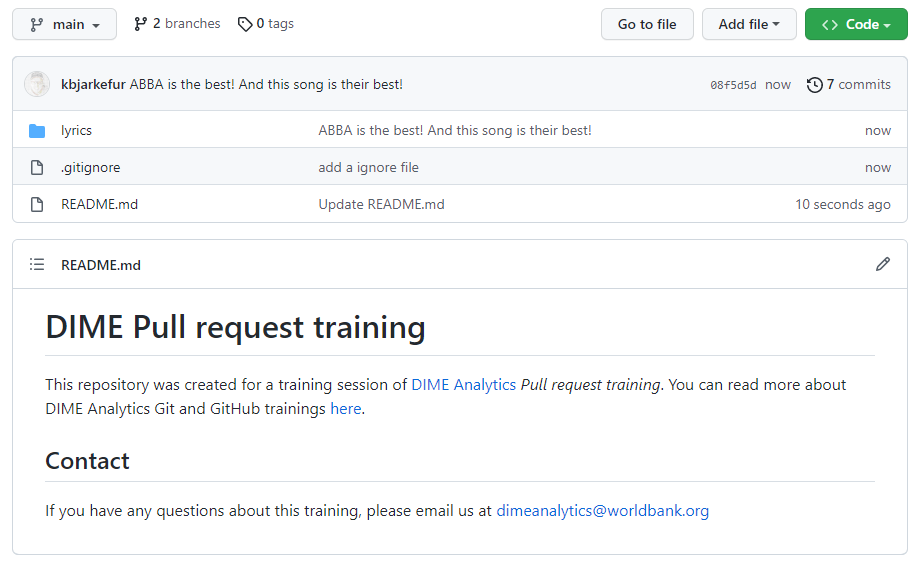
\includegraphics[width=\textwidth]{./img/training-repo.png}
		\end{figure}
	
		\column{.4\textwidth} % Right column and width
		All screenshots in this slide comes from this repo: \trainingRepoURL{}
		
	\end{columns}
\end{frame}

\sectionpic{Part 1: \newline A brief recap to branches}{\rootdir common-resources/img/section-slide-2023}

\begin{frame}
	\frametitle{Brief intro to branches}
	\begin{columns}[c]
		
		\column{.68\textwidth} % Left column and width
		
		Branches are the killer feature of Git. 
		It allows us to approach tasks in a non-linear way,
		which is similar to how human brains
		and especially teams of humans work.
		\vspace{1.5em}	

		Thanks to branches we can (without creating conflicts): 
  \begin{itemize}
      \item Test multiple solutions to a task at the same time
      \item Have multiple people working at different tasks at the same time
  \end{itemize} 
		\vspace{1.5em}
			
		Branches are often visualized in network graphs.
		
		\column{.25\textwidth} % Left column and width
		
		\begin{minipage}[t][6.5cm][t]{\textwidth}
			\begin{figure}
				\centering
				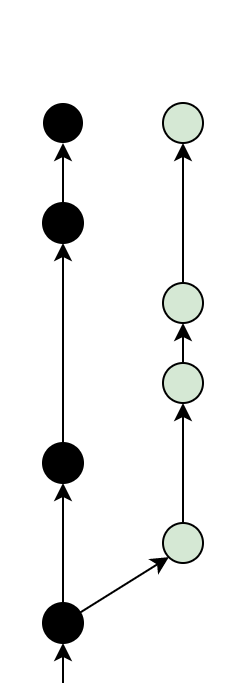
\includegraphics[width=.55\textwidth]{./img/pr-branch.png}
			\end{figure}
		\end{minipage}
		
		\column{.05\textwidth} % Left column and width
		
	\end{columns}
\end{frame}


\begin{frame}
	\frametitle{What are pull requests?}
	\begin{columns}[c]
		
		\column{.68\textwidth} % Left column and width
		
		\textit{Pull requests} (PRs) are part of GitHub, but not part of Git.	
		\vspace{2em}
		
		GitHub is to Git, what Gmail is to email.
		\vspace{2em}
		
		A PR is a request to merge one branch into another,
		and adds great QA and review features before the merge.
		\column{.25\textwidth} % Left column and width
		
		\begin{minipage}[t][6.5cm][t]{\textwidth}
			\begin{figure}
				\centering
				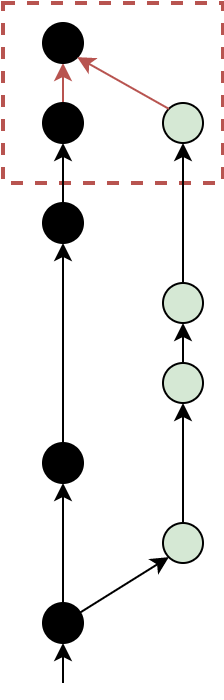
\includegraphics[width=.55\textwidth]{./img/pr-highlight.png}
			\end{figure}
		\end{minipage}
		
		\column{.05\textwidth} % Left column and width
		
	\end{columns}
\end{frame}

\sectionpic{Part 2: \newline The branch-PR-merge cycle}{\rootdir common-resources/img/section-slide-2023}

\begin{frame}
\frametitle{The branch-PR-merge cycle}

	\begin{columns}[c]

		\column{.4\textwidth} % Left column and width
		\large \textbf{Every} data work task in your project should have a \textit{branch-PR-merge} cycle.
		\vspace{.5cm}\newline
		\large The \textit{branch-PR-merge} cycle consists of three stages,
		we will focus on the \textit{work stage} today.

		\column{.6\textwidth} % Right column and width
		\vspace{-.25cm}
		\begin{figure}
			\centering
			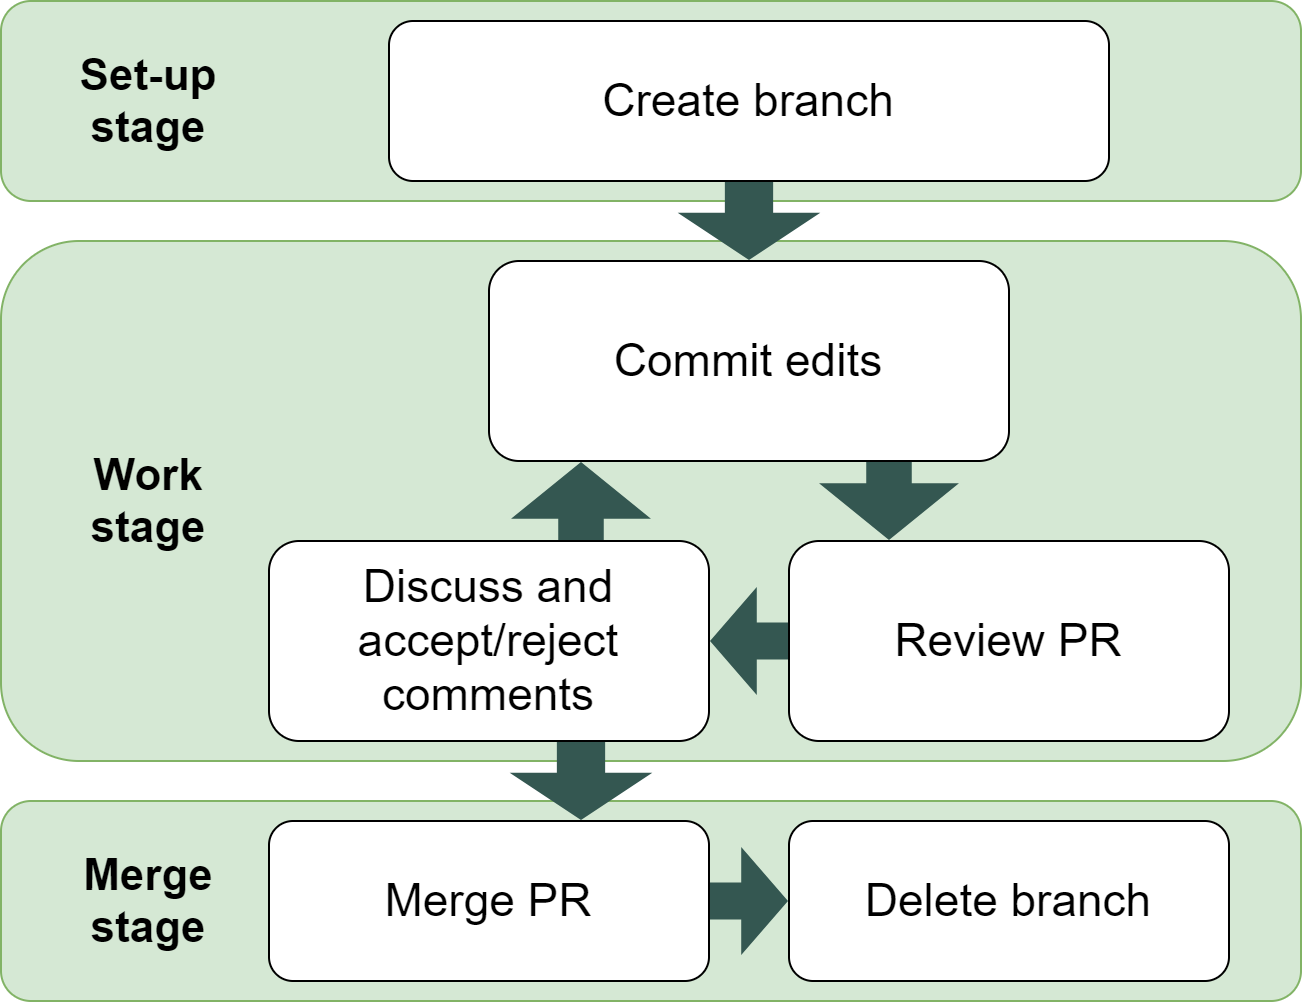
\includegraphics[width=\textwidth]{./img/branch-pr-merge-cycle.png}
		\end{figure}

	\end{columns}
\end{frame}


\begin{frame}
	\frametitle{Set-up Stage}
	\begin{columns}[c]

		\column{.4\textwidth} % Left column and width

		\Large \textbf{SET-UP STAGE:}
		\vspace{.8em}
	
		\normalsize
		Create a branch for this task!
		\vspace{.5cm}\newline
		In Part 3 we will see when and how many branches to create.
		\vspace{.5cm}\newline
		
		\column{.6\textwidth} % Right column and width
		\vspace{-.25cm}
		\begin{figure}
			\centering
			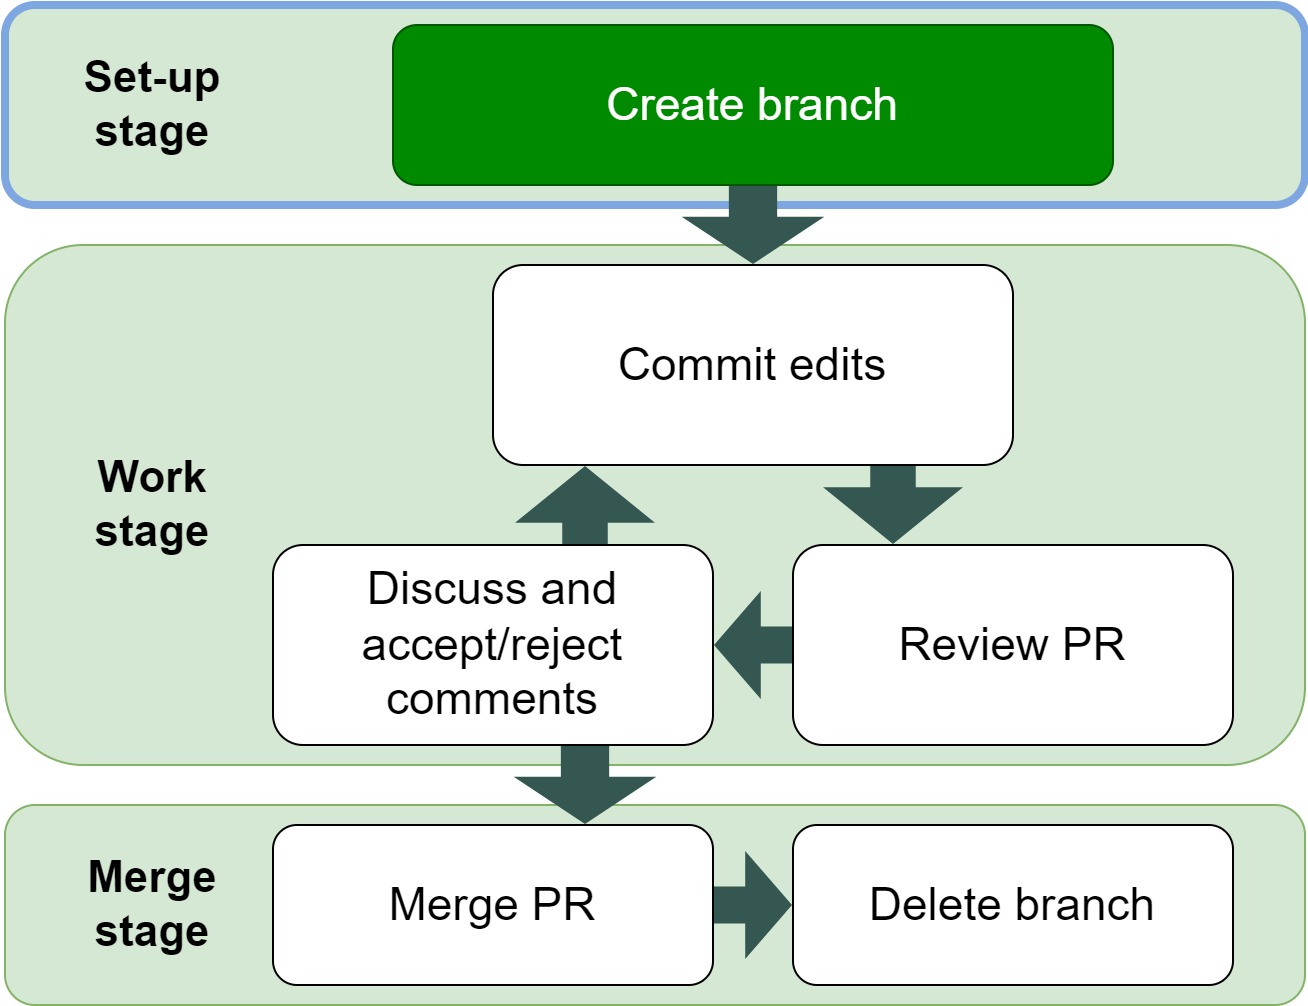
\includegraphics[width=\textwidth]{./img/branch-pr-merge-cycle-S1a.png}
		\end{figure}

	\end{columns}
\end{frame}


\begin{frame}
	\frametitle{Work Stage}
	\begin{columns}[c]
		
		\column{.4\textwidth} % Left column and width
		
		\Large \textbf{WORK STAGE:}
		\vspace{.8em}
		
		\normalsize
		Most time in a branch-PR-merge cycle is spent in the work stage.
		\vspace{.5cm}\newline
		Research teams typically under-utilize features 
		in the \textit{Review} and \textit{Discuss} steps. 
		This is the real added value of PRs.\vspace{.5cm}\newline
		The work stage should be repeated as many times as needed.
		
		\column{.6\textwidth} % Right column and width
		\vspace{-.75cm}
		\begin{figure}
			\centering
			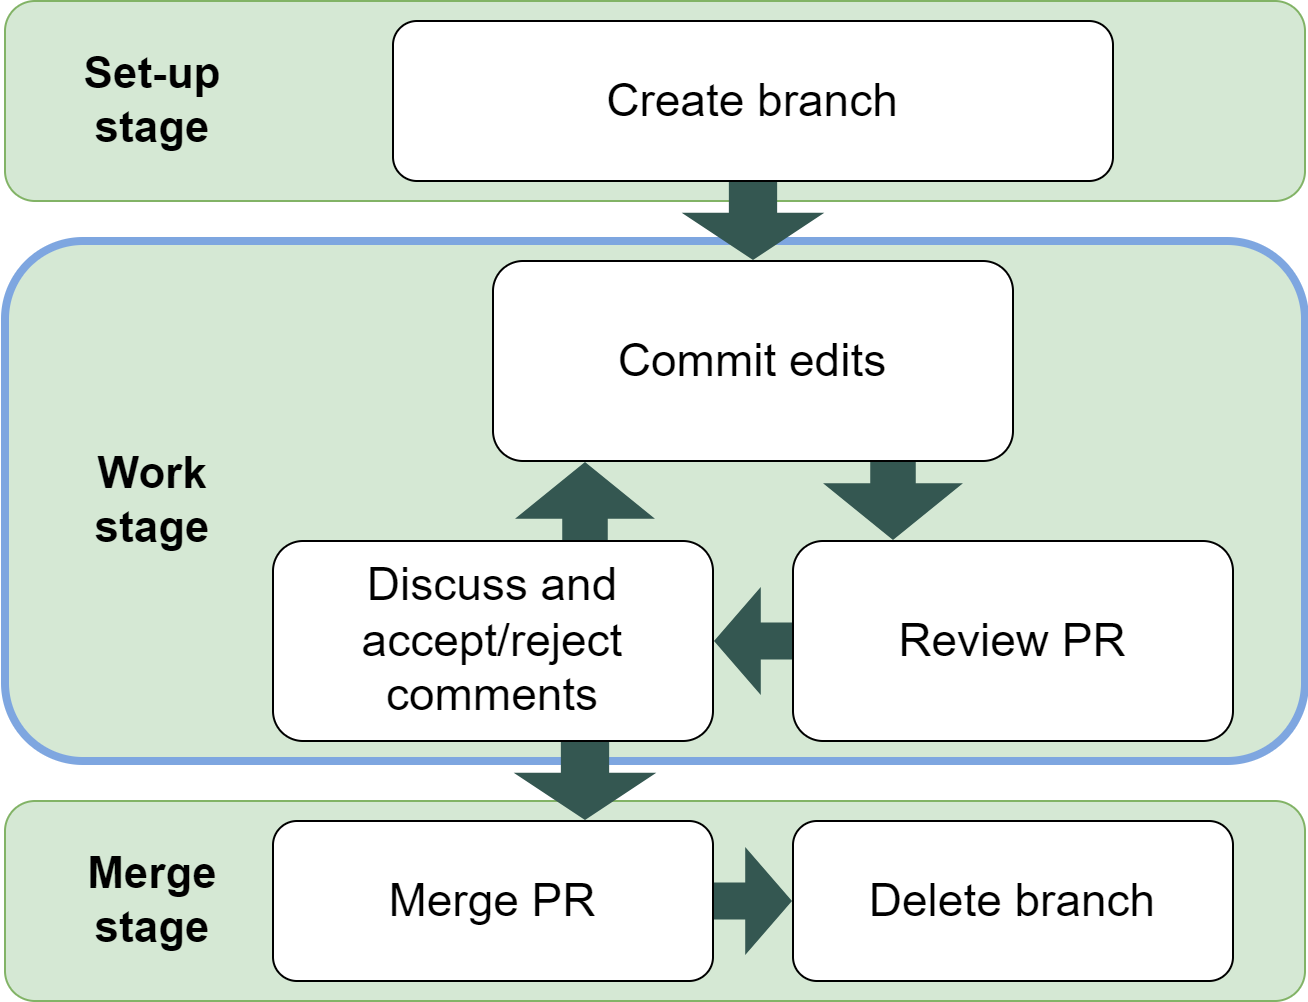
\includegraphics[width=\textwidth]{./img/branch-pr-merge-cycle-S2.png}
		\end{figure}
		
	\end{columns}
\end{frame}

\begin{frame}
	\frametitle{Work Stage: Commit edits}
	\begin{columns}[c]
		
		\column{.4\textwidth} % Left column and width
		
		\normalsize
  		We will call the person making the commits \textit{Author} 
		and the person reviewing the PR \textit{Reviewer}. 
		This can be two people, groups, or one person reviewing their own work.
  \vspace{.5cm}\newline
		In the first step Author working on a task
		commits edits as usual to the new branch.
  \vspace{.5cm}\newline
		The PR must be opened beforeproceeding to the \textit{Review PR} step.
		
		\column{.6\textwidth} % Right column and width
		\vspace{-.75cm}
		\begin{figure}
			\centering
			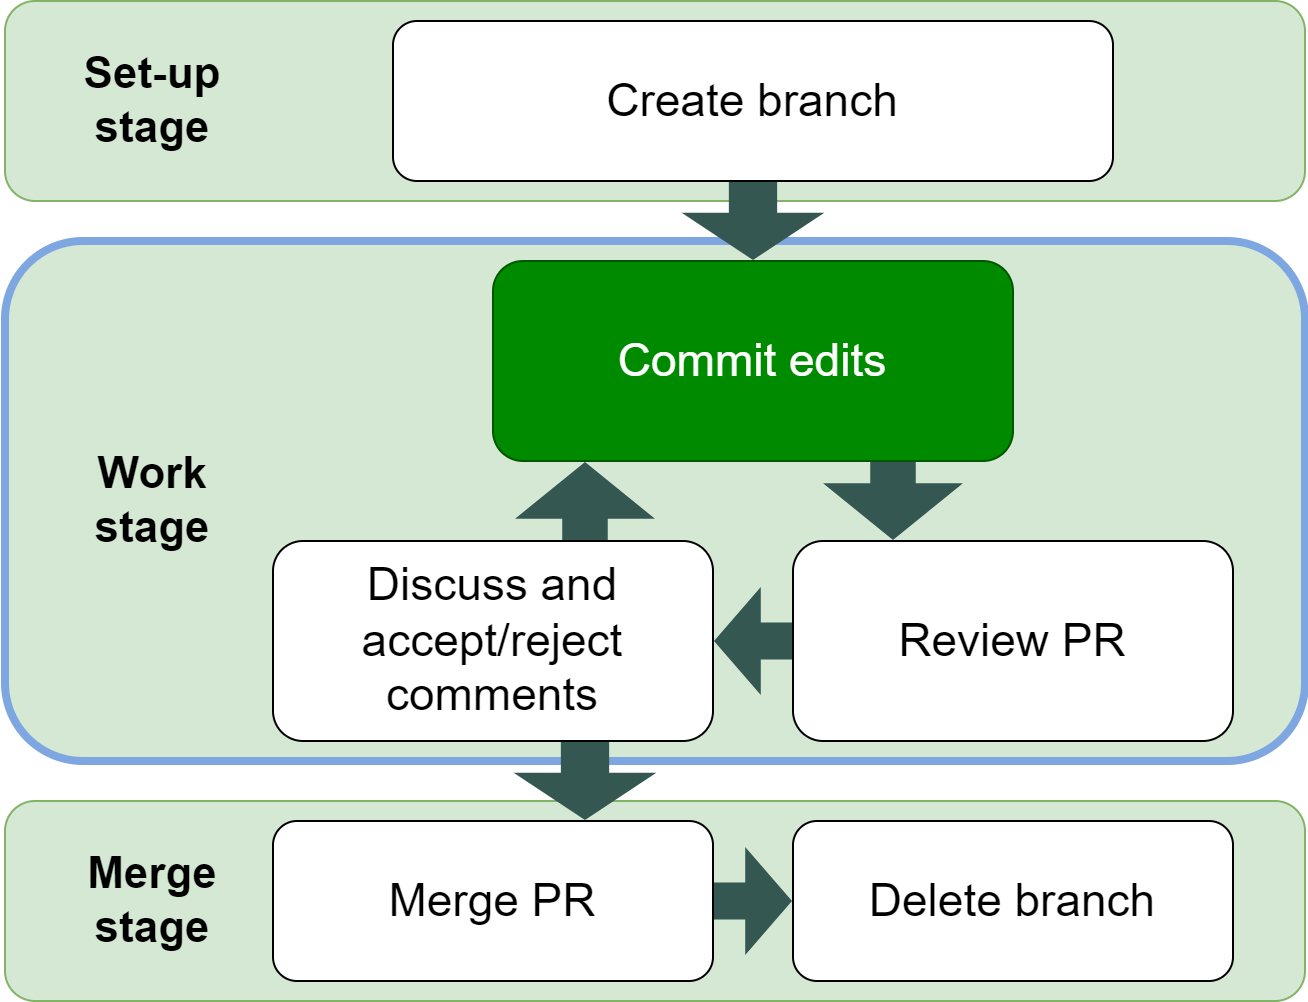
\includegraphics[width=\textwidth]{./img/branch-pr-merge-cycle-S2a.png}
		\end{figure}
		
	\end{columns}
\end{frame}

\begin{frame}
	\frametitle{Create the PR}
	\begin{columns}[c]
		
		\column{.50\textwidth} % Right column and width
		\vspace{-.75cm}
		\begin{figure}
			\centering
			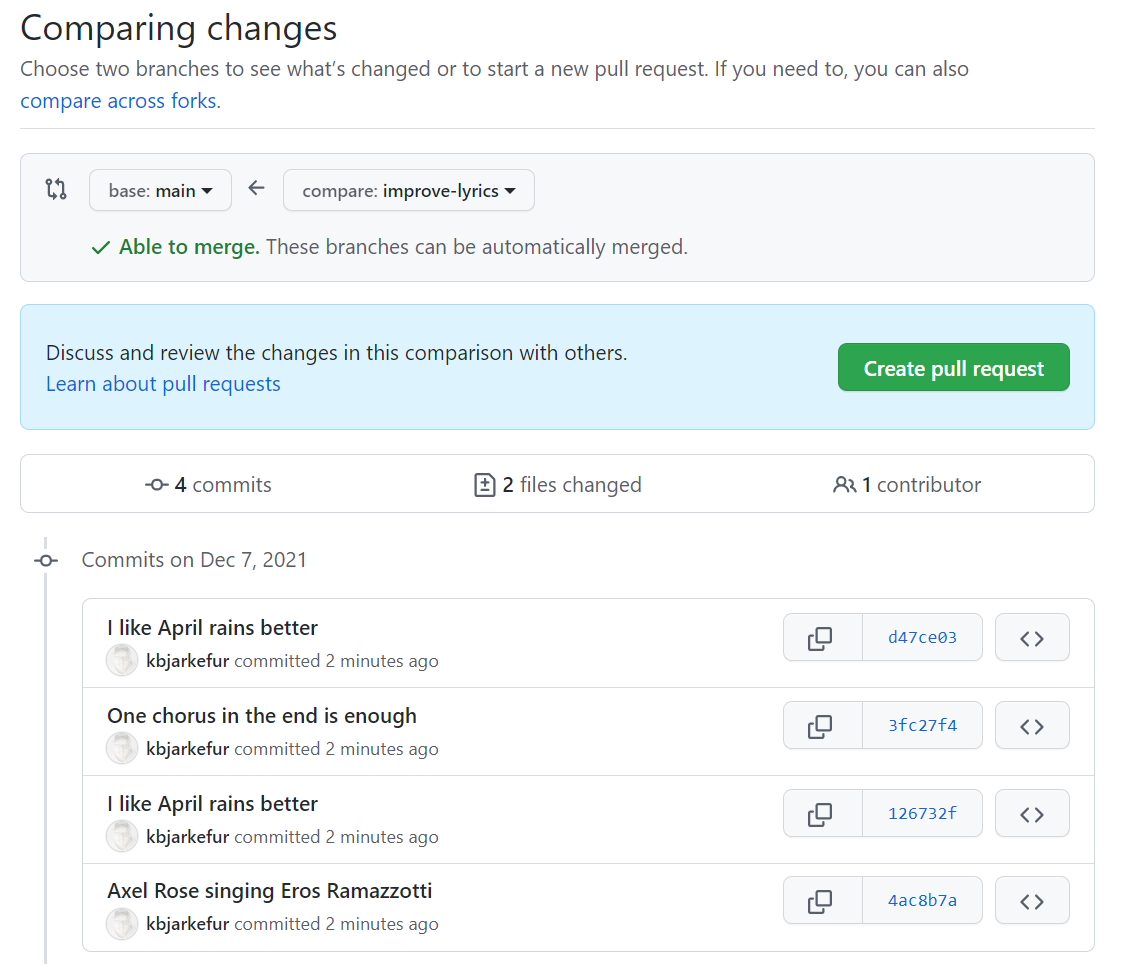
\includegraphics[width=\textwidth]{./img/create-pr-0.png}
		\end{figure}
		
		\column{.50\textwidth} % Left column and width
		\begin{itemize}
			\setlength\itemsep{1em}
		\item Typically done by the Author.
		\item Select the two branches you want to merge:
		    \begin{itemize}
		        \item \textbf{Base branch}: This is the branch into which changes will be merged.
		        \item \textbf{Compare branch}: This is the branch that contains the new changes or features.
		    \end{itemize}
		\item Check the tabs in the \textit{Commits}, \textit{Files changed}, etc., bar to make sure you are creating a PR for the correct branches. Remember, merges can be difficult to revert.
	\end{itemize}
		
	\end{columns}
\end{frame}

\begin{frame}
	\frametitle{Document the PR}
	\begin{columns}[c]
		
		\column{.50\textwidth} % Right column and width
		\begin{figure}
			\centering
			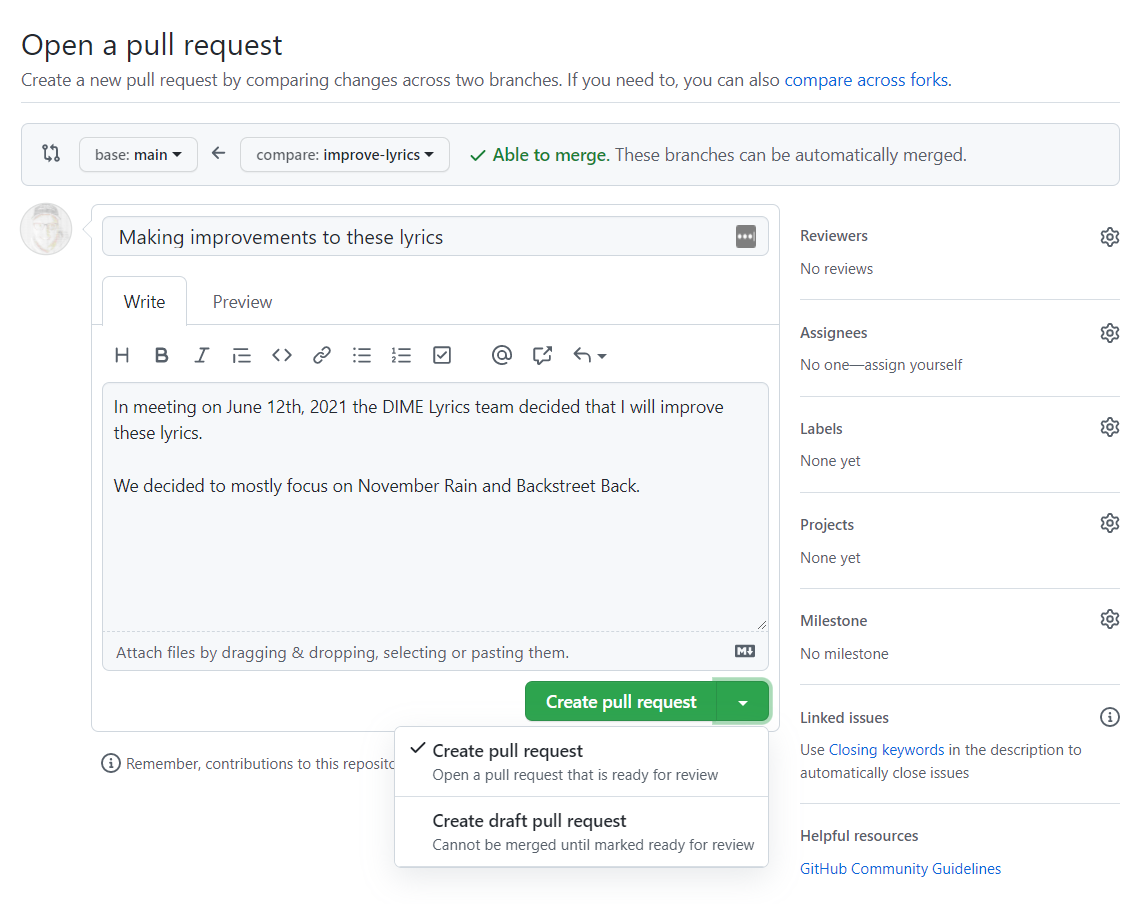
\includegraphics[width=\textwidth]{./img/create-pr-1.png}
		\end{figure}
		
		\column{.50\textwidth} % Left column and width
		\begin{itemize}
			\setlength\itemsep{1em}
			\item Merged PRs are milestones that can be browsed in the future - 
			document these milestones.
			\item Why did the Author work on this task?
			\item Making people reviewers and assignees as well as 
			using labels and projects are neat features, but not necessary.
		\end{itemize}
		
		\vspace{.25cm}
		\footnotesize See this PR at \trainingRepoURLwithParameter{/pull/1}
		
	\end{columns}
\end{frame}


\begin{frame}
	\frametitle{Work Stage : Review PR}
	\begin{columns}[c]
		
		\column{.4\textwidth} % Left column and width
		
		\normalsize
		Review a PR when either: \vspace{.3cm}
		\begin{itemize}
			\item the task is completed.
			\item the Author wants help.
			\item after a set amount of time. 
		\end{itemize}
	
		\vspace{.5cm}

		The PR can be opened as a \textit{Draft PR} already after one commit. 

		
		\column{.6\textwidth} % Right column and width
		\vspace{-.4cm}
		\begin{figure}
			\centering
			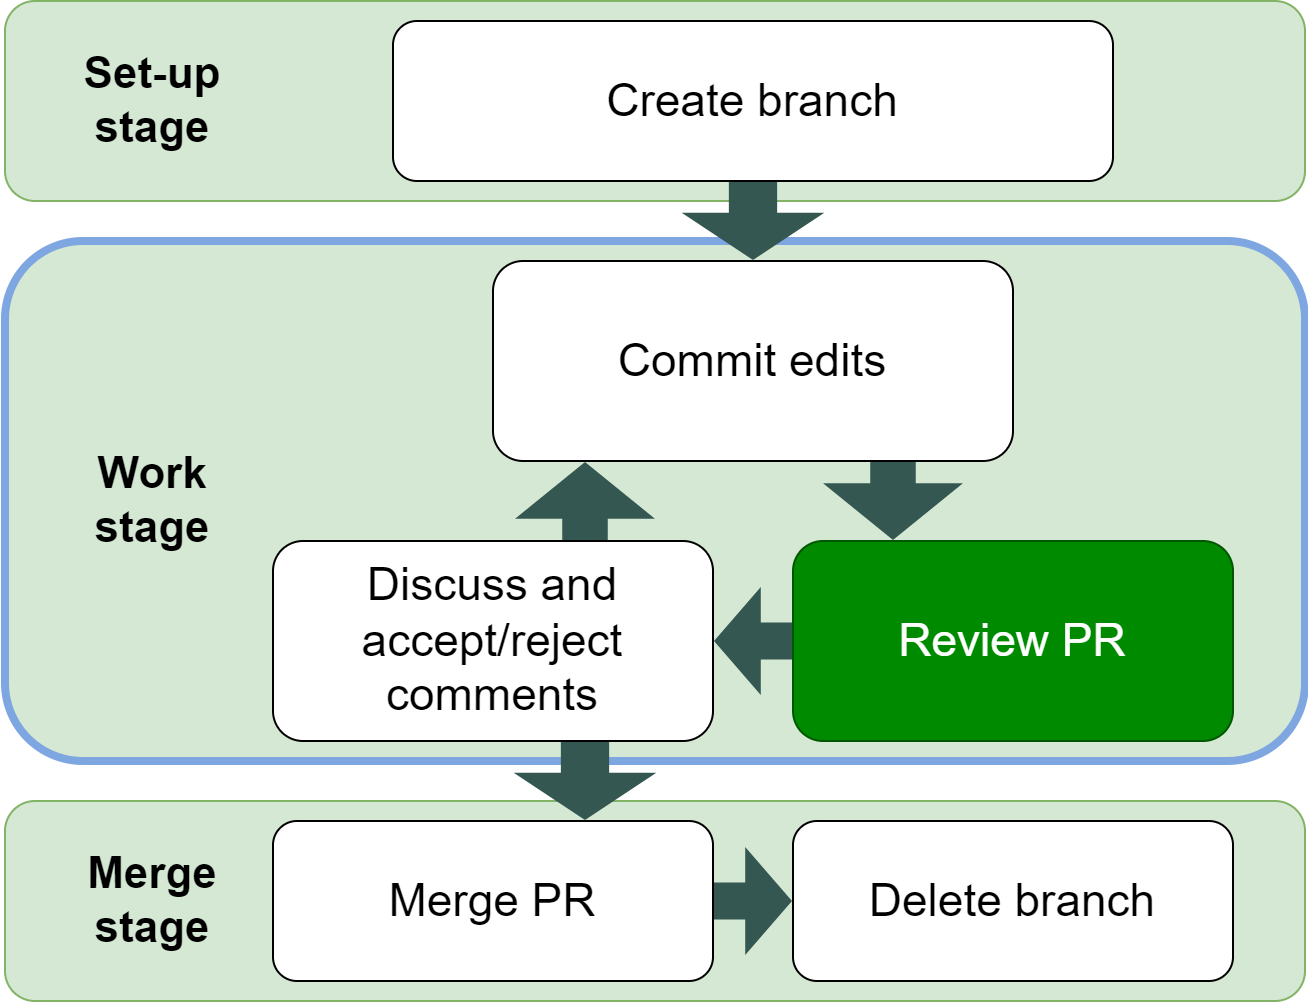
\includegraphics[width=\textwidth]{./img/branch-pr-merge-cycle-S2b.png}
		\end{figure}
		
	\end{columns}
\end{frame}

\begin{frame}
	\frametitle{Overall comments}
	\begin{columns}[c]
		
		\column{.6\textwidth} % Right column and width
		\vspace{-.1cm}
		\begin{figure}
			\centering
			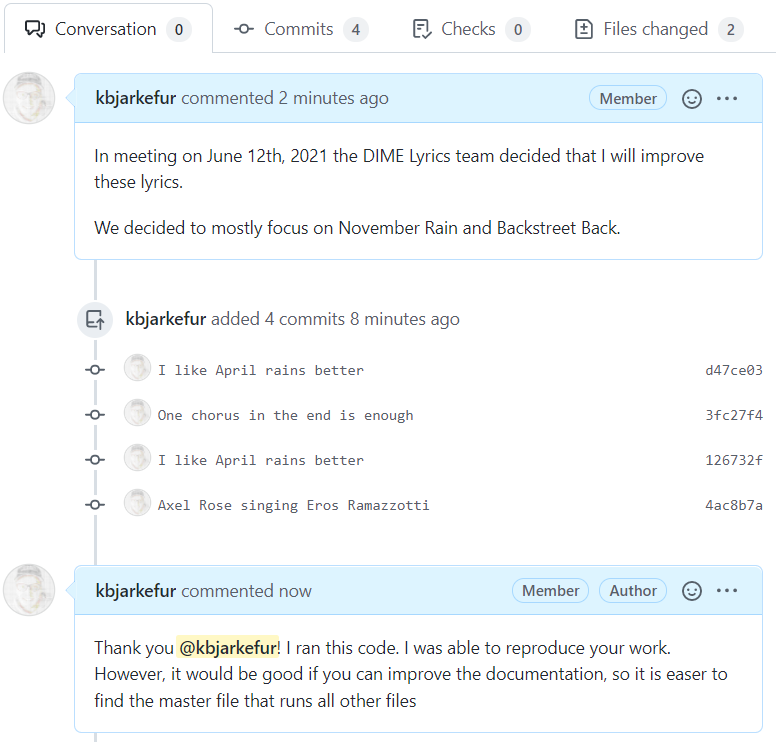
\includegraphics[width=.9\textwidth]{./img/pr-comment.png}
		\end{figure}
		
		\column{.4\textwidth} % Left column and width
		\begin{itemize}
			\setlength\itemsep{1em}
			\item If possible, always start by running the code.
			\item Provide overall comments in the \textit{``Conversation"} tab. Code does or does not run, not possible to follow the code etc.
			\item Tag the Author or Reviewer your comment is meant for.
		\end{itemize}
		
	\end{columns}
\end{frame}

\begin{frame}
	\frametitle{Review the PR}
	\begin{columns}[c]

		\column{.40\textwidth} % Right column and width
		\vspace{-.2cm}
		\begin{figure}
			\centering
			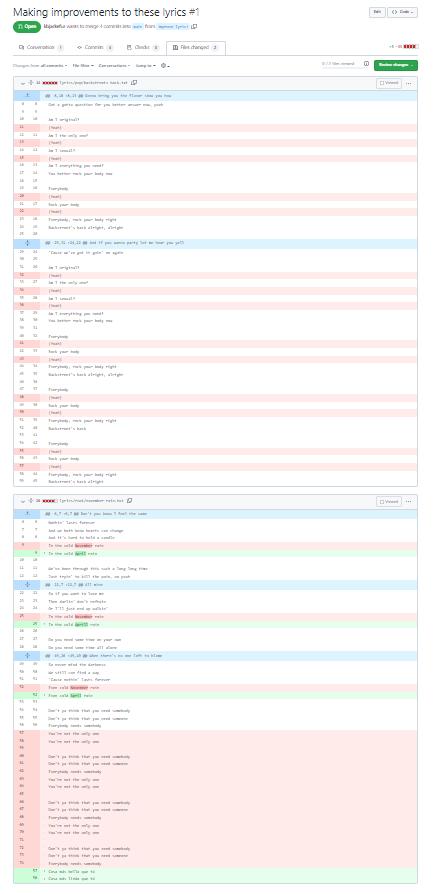
\includegraphics[width=.6\textwidth]{./img/review-1.png}
		\end{figure}

		\column{.60\textwidth} % Left column and width
		\begin{itemize}
			\setlength\itemsep{1.5em}
			\item Next, go to the \textit{``Files changed''} tab
			- this is the summary of all changes in all commits in this PR.
			\item In this tab we make comments to specific lines of code which is always much more useful than overall comments.
		\end{itemize}

	\end{columns}
\end{frame}

\begin{frame}
	\frametitle{Line comments}
	\begin{columns}[c]
		
		\column{.55\textwidth} % Right column and width
		\vspace{-.4cm}
		\begin{figure}
			\centering
			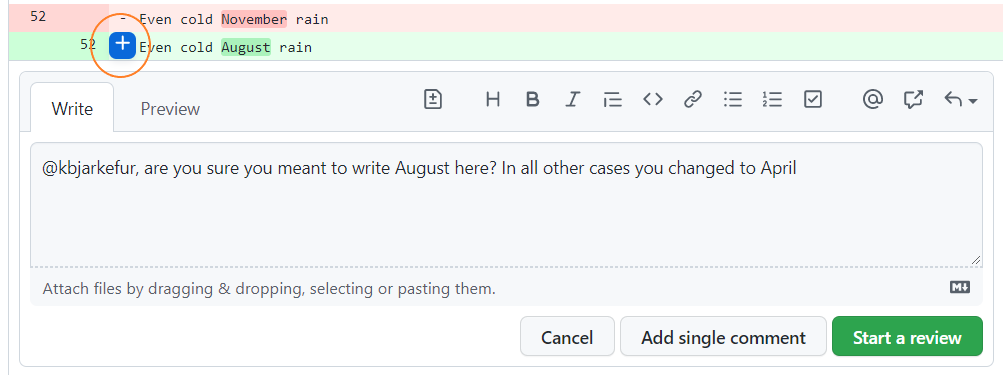
\includegraphics[width=.9\textwidth]{./img/line-comment-1.png}
		\end{figure}
		\vspace{-.3cm}
		\begin{figure}
			\centering
			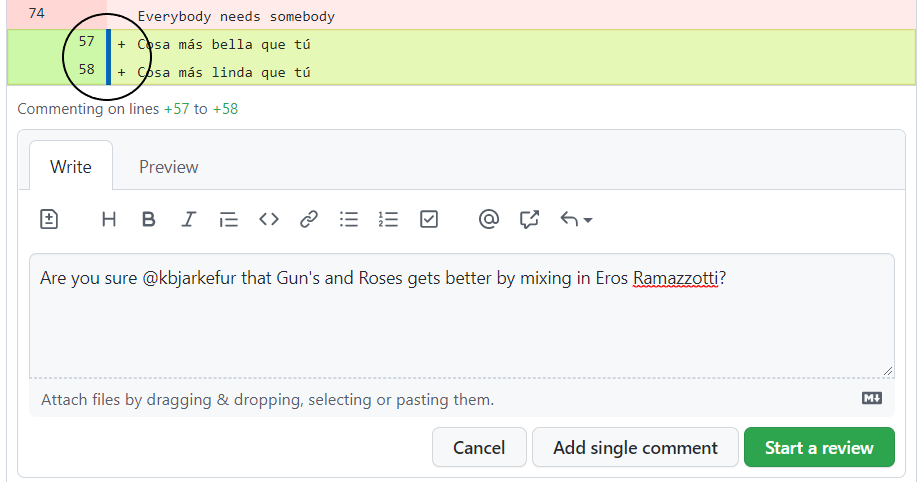
\includegraphics[width=.9\textwidth]{./img/line-comment-2.png}
		\end{figure}
		
		\column{.45\textwidth} % Left column and width
		\begin{itemize}
			\setlength\itemsep{1em}
			\item You can start a thread anywhere in the code in this tab.
			\item \textit{Comment one line}: Hold with the mouse over the line number 
			for a line you want to comment on and click the plus sign - orange circle.
			\item \textit{Comment multiple lines:} Press shift while 
			click-and-drag mouse over multiple lines - black circle.
		\end{itemize}
		
	\end{columns}
\end{frame}

\begin{frame}
	\frametitle{Line suggestions}
	\begin{columns}[c]

		\column{.50\textwidth} % Right column and width
		\vspace{-.6cm}
		\begin{figure}
			\centering
			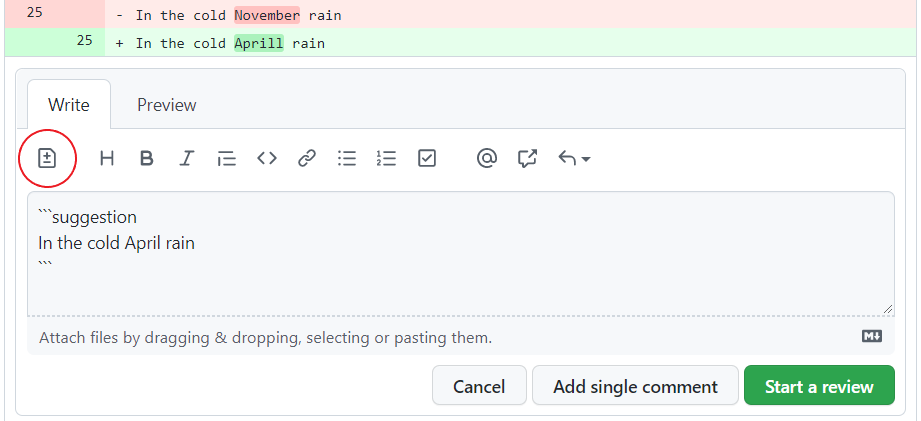
\includegraphics[width=\textwidth]{./img/suggestion-1.png}
		\end{figure}
		\vspace{-.3cm}
		\begin{figure}
			\centering
			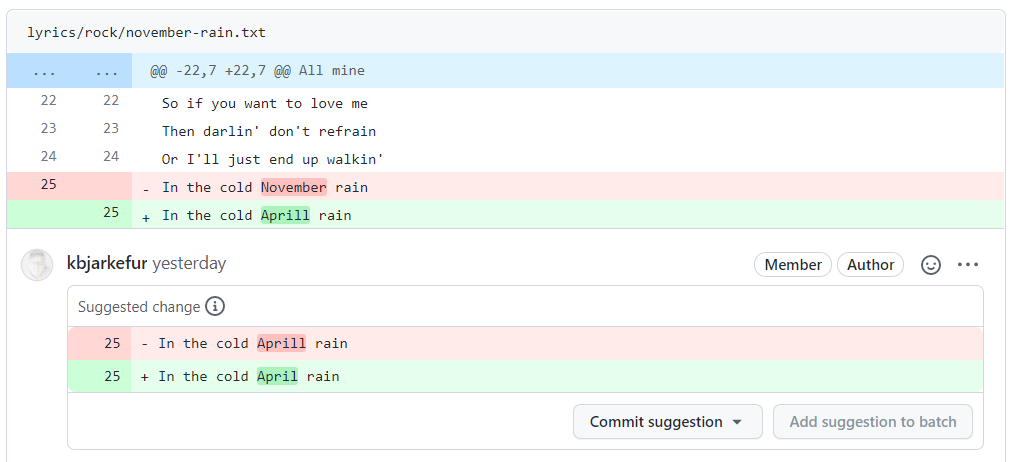
\includegraphics[width=\textwidth]{./img/suggestion-2.png}
		\end{figure}

		\column{.50\textwidth} % Left column and width
		\begin{itemize}
			\setlength\itemsep{.74em}
			\item You can suggest edits to one or multiple lines of code 
			directly in this comment field.
			
			\item Click the suggest code button - red circle - 
			and edit the code that appears.
			
			\item The Author will then see the exact suggestion, 
			and can commit it with the click of a button.
			
			\item Works really well when tweaking the code in the PR,
			but should only be used for smaller edits.
		\end{itemize}

	\end{columns}
\end{frame}

\begin{frame}
	\frametitle{Discuss and accept/reject}
	\begin{columns}[c]

		\column{.35\textwidth} % Left column and width
		\begin{itemize}
			\setlength\itemsep{1em}
			\item The Author and the Reviewer(s) discuss, accept or reject suggestions
			and reply to comments.
			\item The Author, the Reviewer(s)
			and/or anyone else on the project team then
			decide if the work stage needs to be repeated.
		\end{itemize}

		\column{.6\textwidth} % Right column and width
		\vspace{-.4cm}
		\begin{figure}
			\centering
			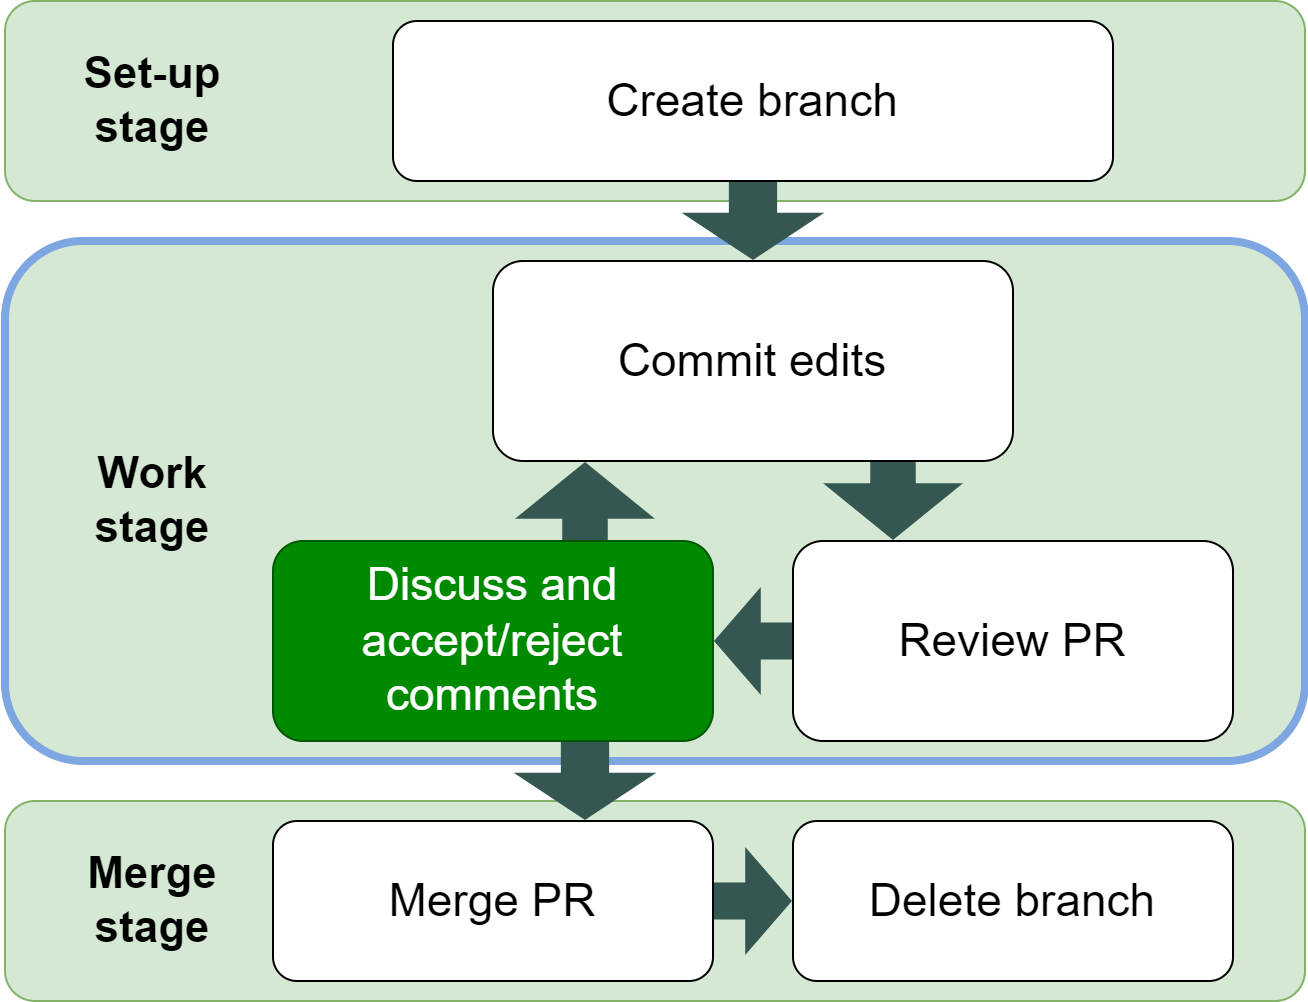
\includegraphics[width=\textwidth]{./img/branch-pr-merge-cycle-S2c.png}
		\end{figure}

	\end{columns}
\end{frame}

\begin{frame}
	\frametitle{Conversation summary}
	\begin{columns}[c]
		
		\column{.4\textwidth} % Right column and width
		\vspace{-.2cm}
		\begin{figure}
			\centering
			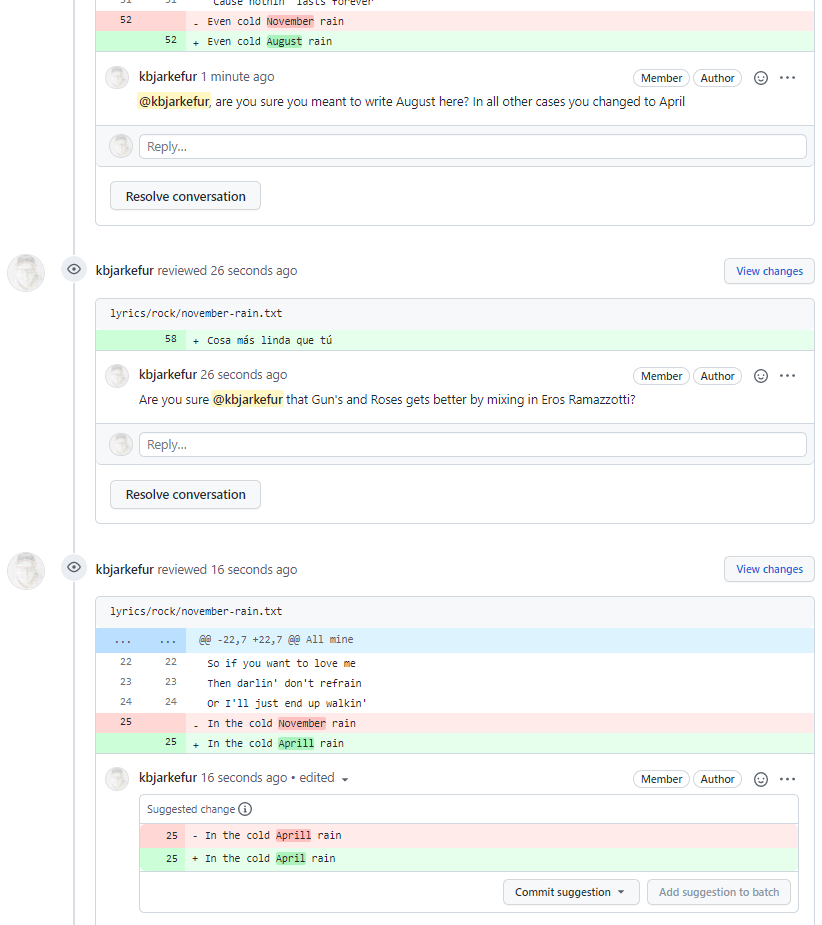
\includegraphics[width=\textwidth]{./img/conversation-summary.png}
		\end{figure}
		
		\column{.60\textwidth} % Left column and width
		\begin{itemize}
			\setlength\itemsep{.68em}
			\item Back in the \textit{``Conversation"} tab, all comments and suggestions are summarized. 
			\item Reply to comments or resolve them by clicking the \textit{``Resolve conversation"} button. 
                \item Resolve suggestions by accepting them with the \textit{``Commit Suggestion"} button or ignore the suggestion by clicking \textit{``Resolve conversation"}.
			\item Keep reviewing the PR until all these comments are resolved.
			\item If possible, always test run the code a final time.
		\end{itemize}
		
	\end{columns}
\end{frame}


\begin{frame}
	\frametitle{Branch-PR-merge }
	\begin{columns}[c]

		\column{.35\textwidth} % Right column and width
		\begin{figure}
			\centering
			
\includegraphics[width=.6\textwidth]{./img/qa.png}
		\end{figure}

		\column{.55\textwidth} % Left column and width
		\begin{itemize}
			\setlength\itemsep{1em}
			\item After responding to all suggestions and comments, 
   the team should discuss whether the task is completed or requires further work.
			\item Repeat the work stage 
			if significant work is still required.
			\item Move on to the merge stage 
			only when the task is complete and 
			the team agrees the code is high-quality.
		\end{itemize}

	\end{columns}
\end{frame}


\begin{frame}
	\frametitle{Merge Stage}
	\begin{columns}[c]
		
		\column{.4\textwidth} % Left column and width
		
		\Large \textbf{MERGE STAGE:}
		\vspace{.8em}
		
		\normalsize
		The last stage of the \textit{branch-PR-merge} cycle is to merge the PR
		once everyone has agreed to the suggested changes.
		\vspace{.5cm}\newline
		Always delete the old branch - recreate that branch from the \textit{base} branch
		if you want to keep working in a branch with the same name.
		
		\column{.6\textwidth} % Right column and width
		\vspace{-.75cm}
		\begin{figure}
			\centering
			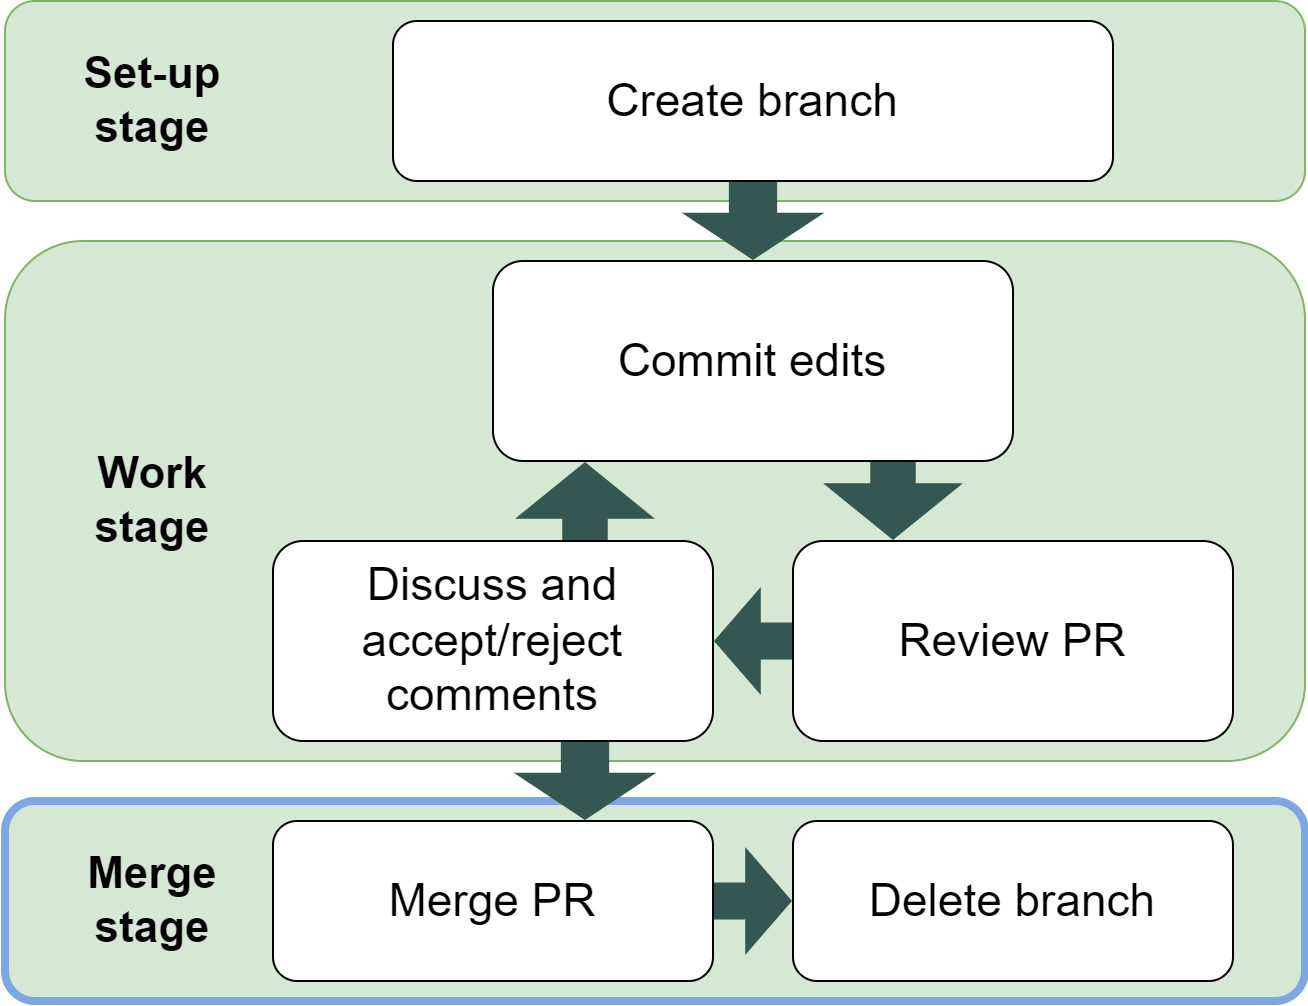
\includegraphics[width=\textwidth]{./img/branch-pr-merge-cycle-S3.png}
		\end{figure}
		
	\end{columns}
 
\end{frame}


\begin{frame}
	\frametitle{Exercise: Apply the branch-PR-merge cycle}
		\begin{itemize}
		\item Objective: Practice the complete branch-PR-merge cycle.  We will use our \exerciseRepoURL{} repository.
		\item Tasks:
		\begin{enumerate}
			\item \textbf{Set-Up Stage:} Create and switch to a branch named "your\_name\_session2".
			\item \textbf{Work Stage:}
			\begin{itemize}
				\item Commit Edits: Add or modify a song in the "lyrics" directory. Commit your changes and push them to GitHub.
				\item Review PR: Open a pull request against the main branch. Pair up to review each other’s PRs, focusing on constructive feedback using GitHub’s comment and review tools.
				\item Discuss Comments: Engage with your partner's feedback on your PR—discuss, accept, or reject suggestions.
			\end{itemize}
			\item \textbf{Merge Stage:} Ensure all feedback has been addressed. After receiving peer approval, merge your pull request.
		\end{enumerate}
	\end{itemize}
\end{frame}


\sectionpic{Part 3: \newline Gitflow - When, how and how much to branch}{\rootdir common-resources/img/section-slide-2023}

\begin{frame}
	\frametitle{The network graph}

	\vspace{-.5cm}
	\begin{minipage}[t][5cm][t]{\textwidth}
		\begin{figure}
			\centering
			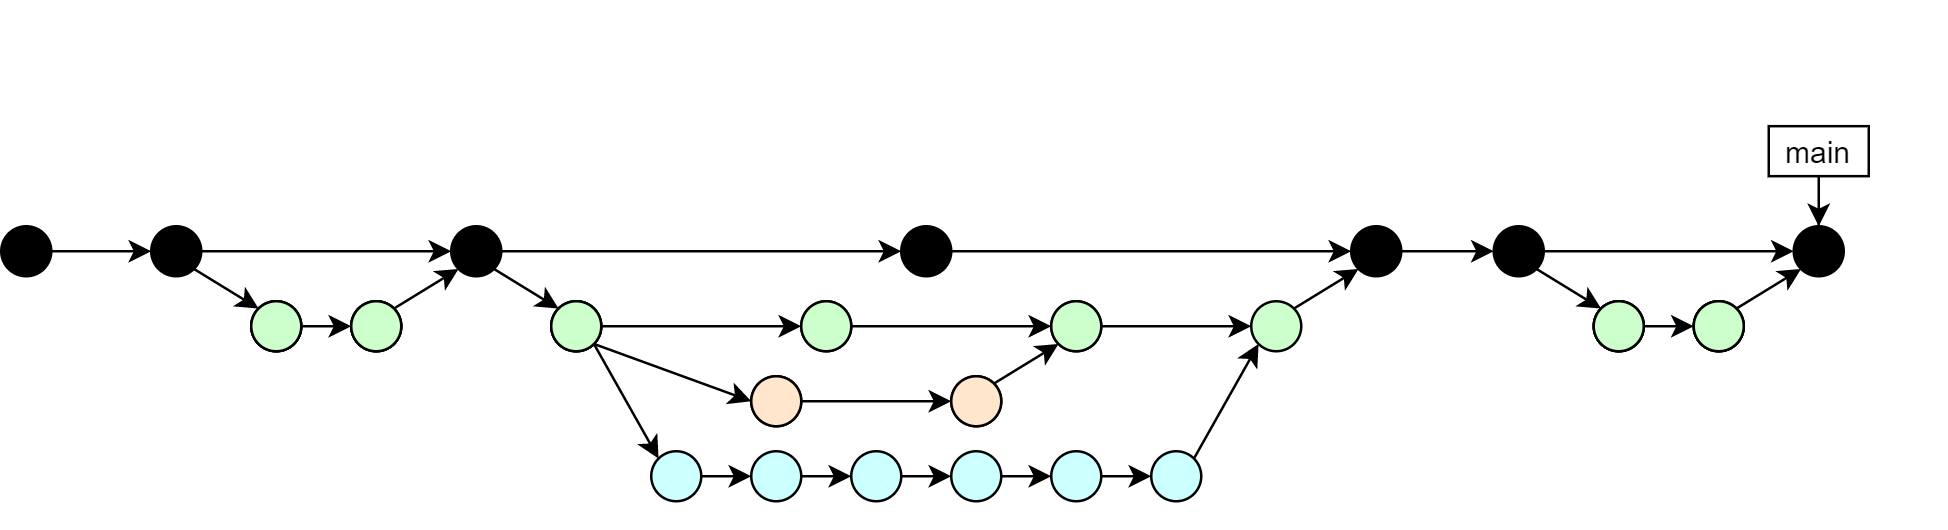
\includegraphics[width=\textwidth]{./img/dime-gitflow-network.png}
		\end{figure}
	\end{minipage}

	\vspace{-.5cm}
	\begin{minipage}[t][5cm][t]{\textwidth}
		\begin{itemize}
			\setlength\itemsep{.5em}
			\item A typical git network graph - each dot is a commit.
			\item Several branches have been opened and merged,
			but currently only the \textit{main} branch is open.
		\end{itemize}
	\end{minipage}

\end{frame}

\begin{frame}
	\frametitle{Gitflow}
	\begin{columns}[c]

		\column{.65\textwidth} % Left column and width
		\begin{itemize}
			\setlength\itemsep{.5em}
			\item \textbf{Gitflow} is an idea or a philosophy 
			of how to organize work in git - it is not a software you install.
			\item It is developed by computer scientists and
			you will find a lot of resources for it online.
			\item We will present a simplified version adapted for research
			\item Two branch types (later we add a third type):
			\begin{itemize}
				\item The \textbf{main branch} (formerly master branch)
				- should never be worked in directly.
				\item \textbf{Feature branches} - this is where all work should be done.
			\end{itemize}
		\end{itemize}

		\column{.35\textwidth} % Right column and width
		\vspace{-.75cm}
		\begin{figure}
			\centering
			
\includegraphics[width=.75\textwidth]{./img/organization.png}
		\end{figure}
	\end{columns}
\end{frame}



\begin{frame}
	\frametitle{Simple branch-PR-merge cycle}

	\huge\centering \textbf{Simple branch-PR-merge cycle}

\end{frame}


\begin{frame}
	\frametitle{Start a branch-PR-merge cycle}

	\vspace{-.5cm}
	\begin{minipage}[t][5cm][t]{\textwidth}
		\begin{figure}
			\centering
			\includegraphics[width=\textwidth]{./img/dime-gitflow-network-0.png}
		\end{figure}
	\end{minipage}

	\vspace{-.5cm}
	\begin{minipage}[t][5cm][t]{\textwidth}
		\begin{itemize}
			\setlength\itemsep{.5em}
			\item This can either be the beginning of a repo
			or at a point where all previous branches were merged
			to the main branch.
			\item Let's say your next task is to set up folders
			- apply the \textit{branch-PR-merge} cycle.
		\end{itemize}
	\end{minipage}

\end{frame}

\begin{frame}
	\frametitle{Set up stage - 1}

	\vspace{-.5cm}
	\begin{minipage}[t][5cm][t]{\textwidth}
		\begin{figure}
			\centering
			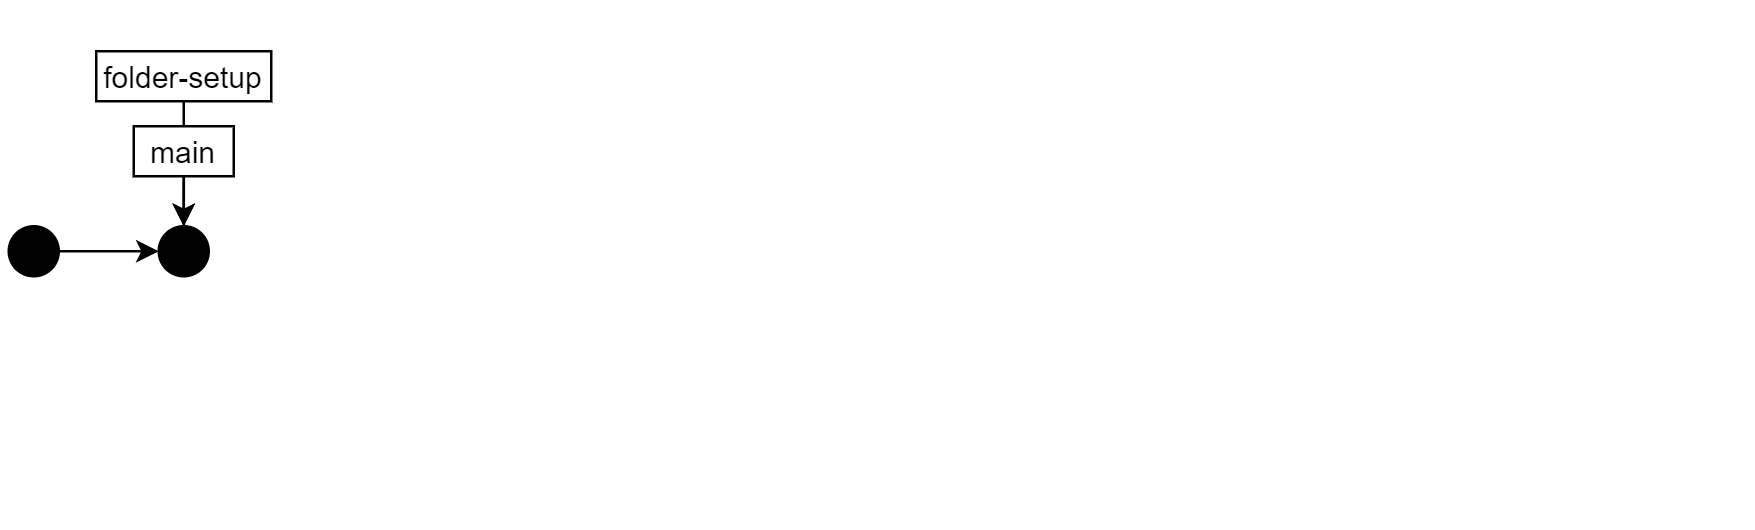
\includegraphics[width=\textwidth]{./img/dime-gitflow-network-1-0.png}
		\end{figure}
	\end{minipage}

	\vspace{-.5cm}
	\begin{minipage}[t][5cm][t]{\textwidth}
		\begin{itemize}
			\setlength\itemsep{.5em}
			\item Create a new \textit{feature} branch at the point
			where you want the the \textit{branch-PR-merge} cycle
			to start from.
			\item Two branches pointing to the same commit
			are identical by definition.
		\end{itemize}
	\end{minipage}

\end{frame}


\begin{frame}
	\frametitle{Set up stage - 2}

	\vspace{-.5cm}
	\begin{minipage}[t][5cm][t]{\textwidth}
		\begin{figure}
			\centering
			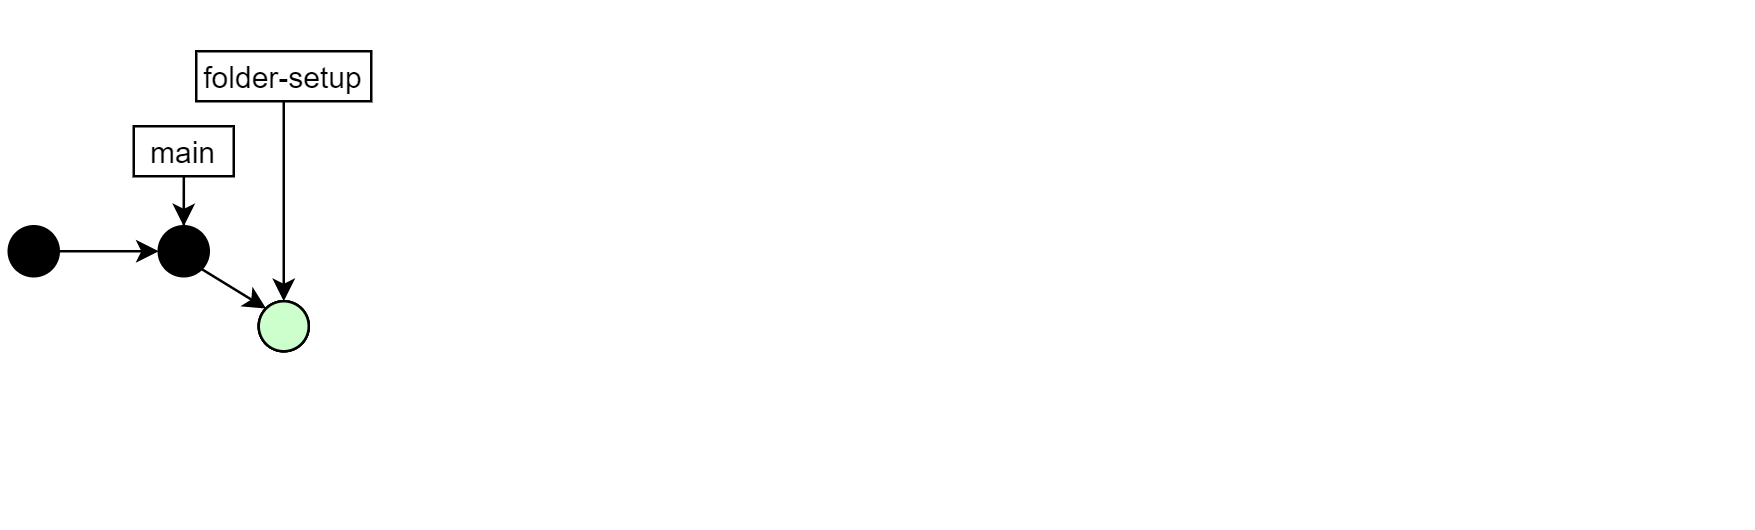
\includegraphics[width=\textwidth]{./img/dime-gitflow-network-1-1.png}
		\end{figure}
	\end{minipage}

	\vspace{-.5cm}
	\begin{minipage}[t][5cm][t]{\textwidth}
		\begin{itemize}
			\setlength\itemsep{.5em}
			\item The Author starts working on the task in the new branch.
			\item As soon as one commit is made you can open a new PR 
			where this task can be reviewed and discussed - great case for a draft PR.
		\end{itemize}
	\end{minipage}

\end{frame}

\begin{frame}
	\frametitle{Work stage}

	\vspace{-.5cm}
	\begin{minipage}[t][5cm][t]{\textwidth}
		\begin{figure}
			\centering
			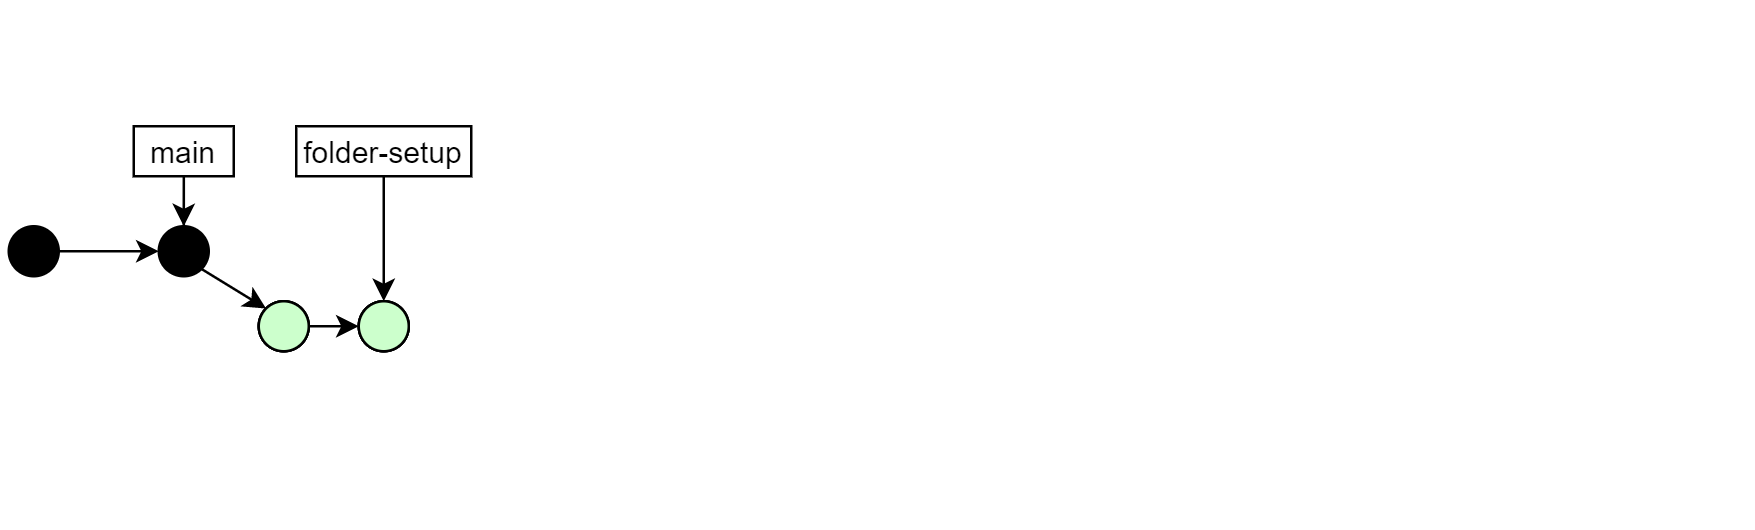
\includegraphics[width=\textwidth]{./img/dime-gitflow-network-1-2.png}
		\end{figure}
	\end{minipage}

	\vspace{-.5cm}
	\begin{minipage}[t][5cm][t]{\textwidth}
		\begin{itemize}
			\setlength\itemsep{.5em}
			\item Complete the task using one or many commits
			- in this example, only one more commit was needed.
			\item Assign someone to review the PR
			- iterate the work stage of the branch-PR-merge cycle until everyone is satisfied.
		\end{itemize}
	\end{minipage}

\end{frame}

\begin{frame}
	\frametitle{Merge stage}

	\vspace{-.5cm}
	\begin{minipage}[t][5cm][t]{\textwidth}
		\begin{figure}
			\centering
			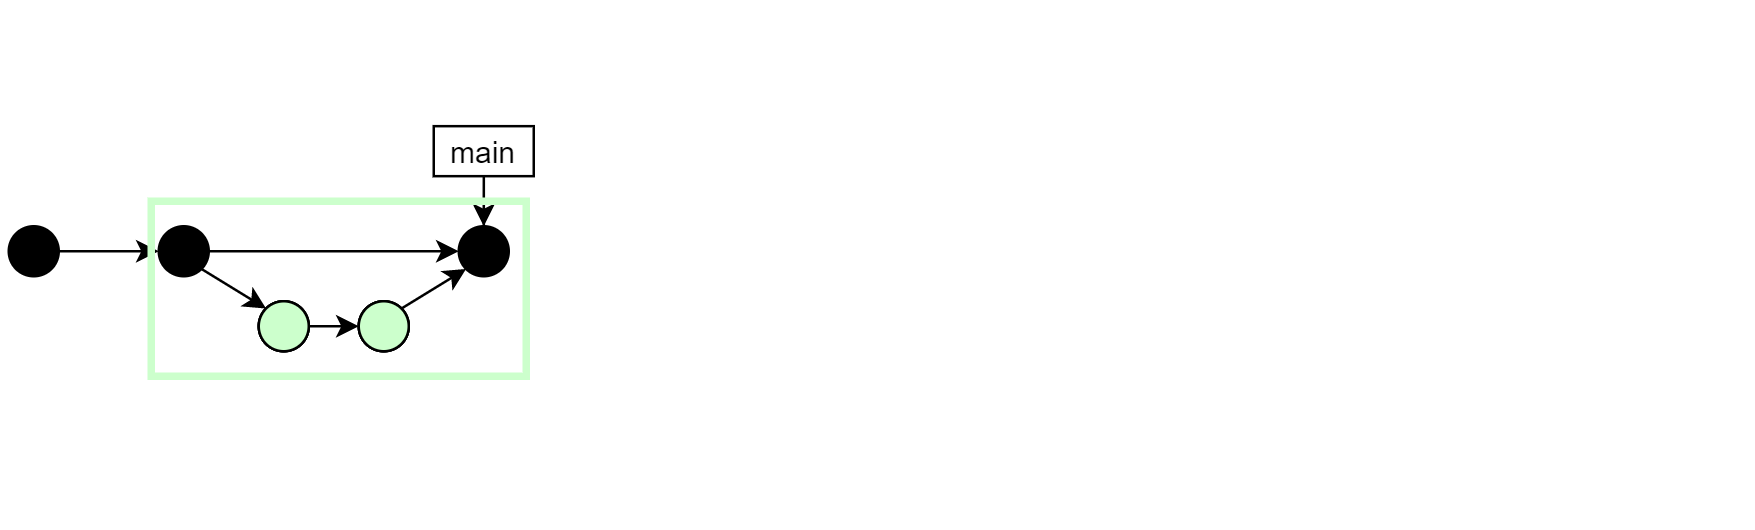
\includegraphics[width=\textwidth]{./img/dime-gitflow-network-1-3.png}
		\end{figure}
	\end{minipage}

	\vspace{-.5cm}
	\begin{minipage}[t][5cm][t]{\textwidth}
		\begin{itemize}
			\setlength\itemsep{.5em}
			\item Merge the PR and delete the \textit{feature} branch.
			\item The green box represents
			a full \textit{branch-PR-merge} cycle in the network graph.
		\end{itemize}
	\end{minipage}

\end{frame}

\begin{frame}
	\frametitle{Nested branch-PR-merge cycles}

	\huge\centering \textbf{Nested branch-PR-merge cycles}

\end{frame}

\begin{frame}
	\frametitle{Nested branch-PR-merge cycles}
	\begin{columns}[c]

		\column{.65\textwidth} % Left column and width
		\begin{itemize}
			\setlength\itemsep{.5em}
			\item Many high-level tasks are not simple
			- many team members working over multiple months.
			\item Cleaning the baseline data,
			for example, is one big task composed of many smaller tasks
			\item Solve this by using nested \textit{branch-PR-merge} cycles
			\item Third type of branch: \textbf{Develop branch}
			- a branch that is a high-level task that
			will have several \textit{feature} branches
		\end{itemize}

		\column{.35\textwidth} % Right column and width

		\begin{figure}
			\centering
			
\includegraphics[width=.65\textwidth]{./img/team-challenge.png}
		\end{figure}
	\end{columns}
\end{frame}

\begin{frame}
	\frametitle{Create a develop branch}

	\vspace{-.5cm}
	\begin{minipage}[t][5cm][t]{\textwidth}
		\begin{figure}
			\centering
			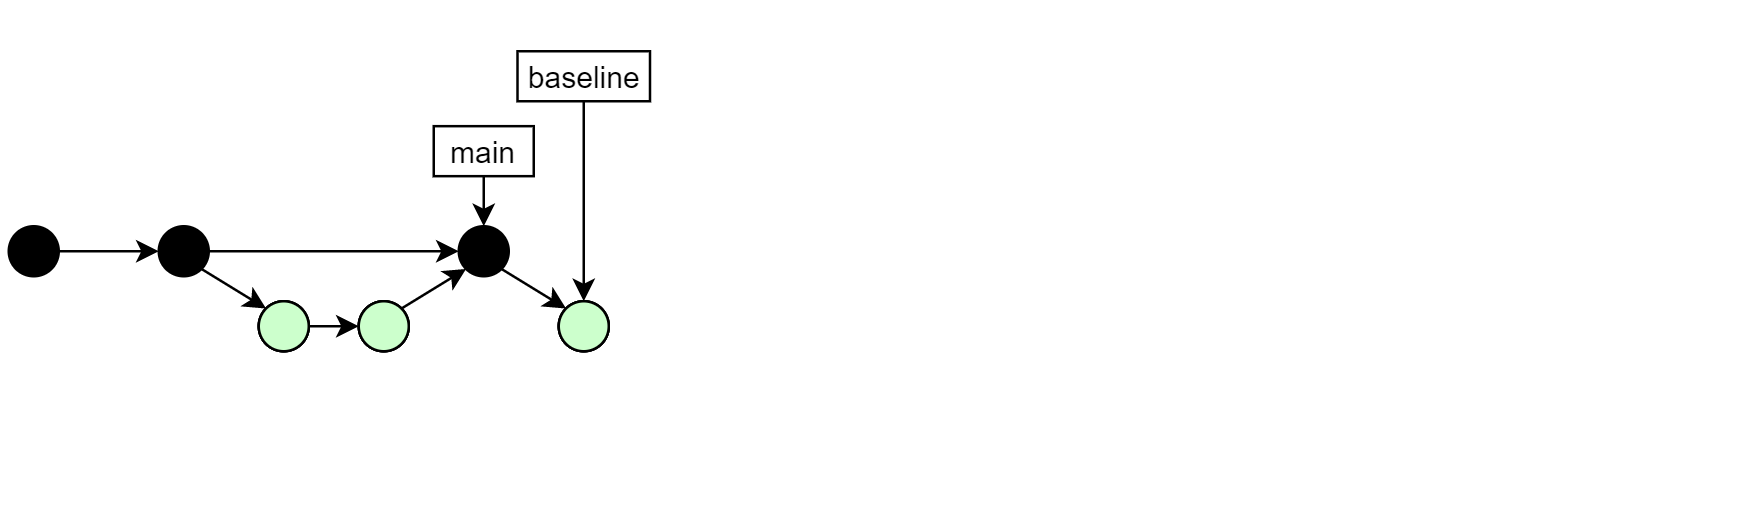
\includegraphics[width=\textwidth]{./img/dime-gitflow-network-2-1.png}
		\end{figure}
	\end{minipage}

	\vspace{-.5cm}
	\begin{minipage}[t][5cm][t]{\textwidth}
		\begin{itemize}
			\setlength\itemsep{1em}
			\item Create a \textit{develop} branch
			- name it after the high-level task.
			\item Include the name of the \textit{develop} branch as prefix
			to all \textit{feature} branches off it.
		\end{itemize}
	\end{minipage}
\end{frame}

\begin{frame}
	\frametitle{Create feature branches of the develop branch}

	\vspace{-.5cm}
	\begin{minipage}[t][5cm][t]{\textwidth}
		\begin{figure}
			\centering
			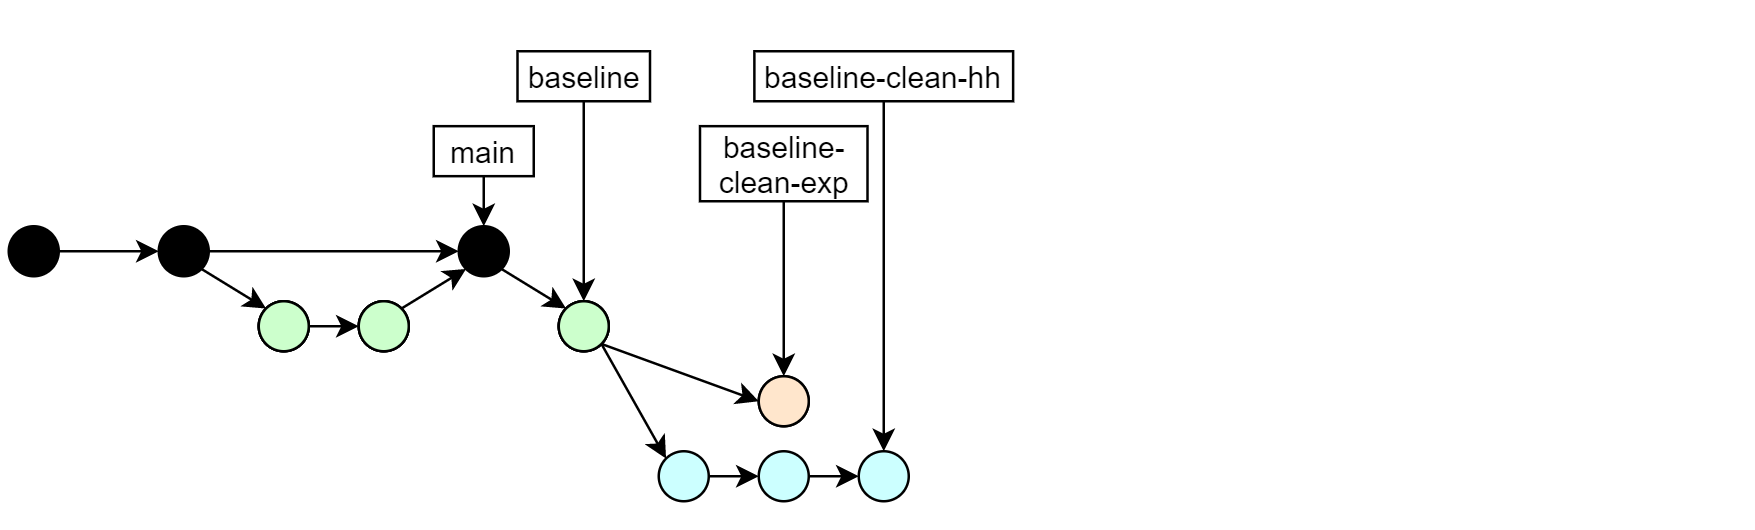
\includegraphics[width=\textwidth]{./img/dime-gitflow-network-2-2.png}
		\end{figure}
	\end{minipage}

	\vspace{-.5cm}
	\begin{minipage}[t][5cm][t]{\textwidth}
		\begin{itemize}
			\setlength\itemsep{.5em}
			\item Create as many \textit{feature} branches off
			the \textit{develop} branch as you need.
			\item Split up the high-level task in as many smaller tasks as needed
			- try to split up tasks until each is small enough
			for one person to complete in max a week or two.
			\item Create new \textit{feature} branches off
			the \textit{develop} branch even after it progresses.
		\end{itemize}
	\end{minipage}
\end{frame}

\begin{frame}
	\frametitle{Work in the branches}

	\vspace{-.5cm}
	\begin{minipage}[t][5cm][t]{\textwidth}
		\begin{figure}
			\centering
			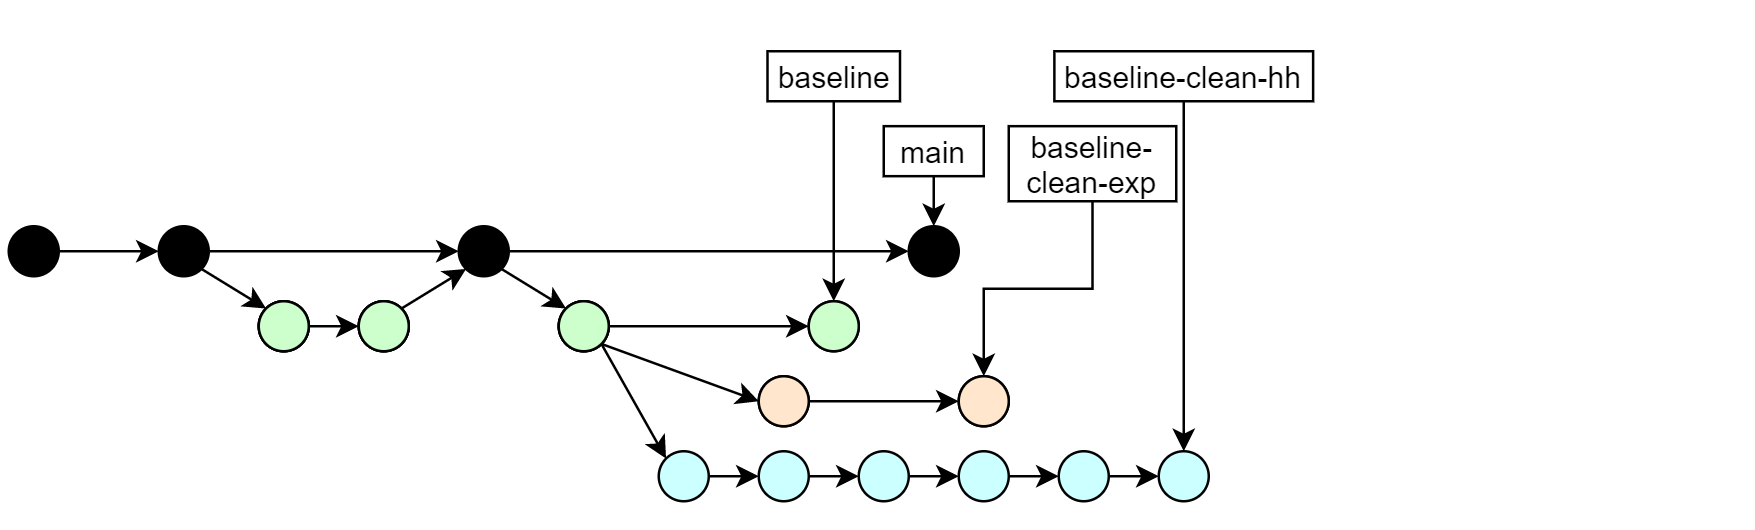
\includegraphics[width=\textwidth]{./img/dime-gitflow-network-2-3.png}
		\end{figure}
	\end{minipage}

	\vspace{-.5cm}
	\begin{minipage}[t][5cm][t]{\textwidth}
		\begin{itemize}
			\setlength\itemsep{.5em}
			\item The Author keeps working on the \textit{feature} branches until
			the task is done.
			\item When a task is complete: assign a reviewer
			- make comments/suggestions - accept/reject/discuss.
		\end{itemize}
	\end{minipage}
\end{frame}

\begin{frame}
	\frametitle{Merge a feature branch}

	\vspace{-.5cm}
	\begin{minipage}[t][5cm][t]{\textwidth}
		\begin{figure}
			\centering
			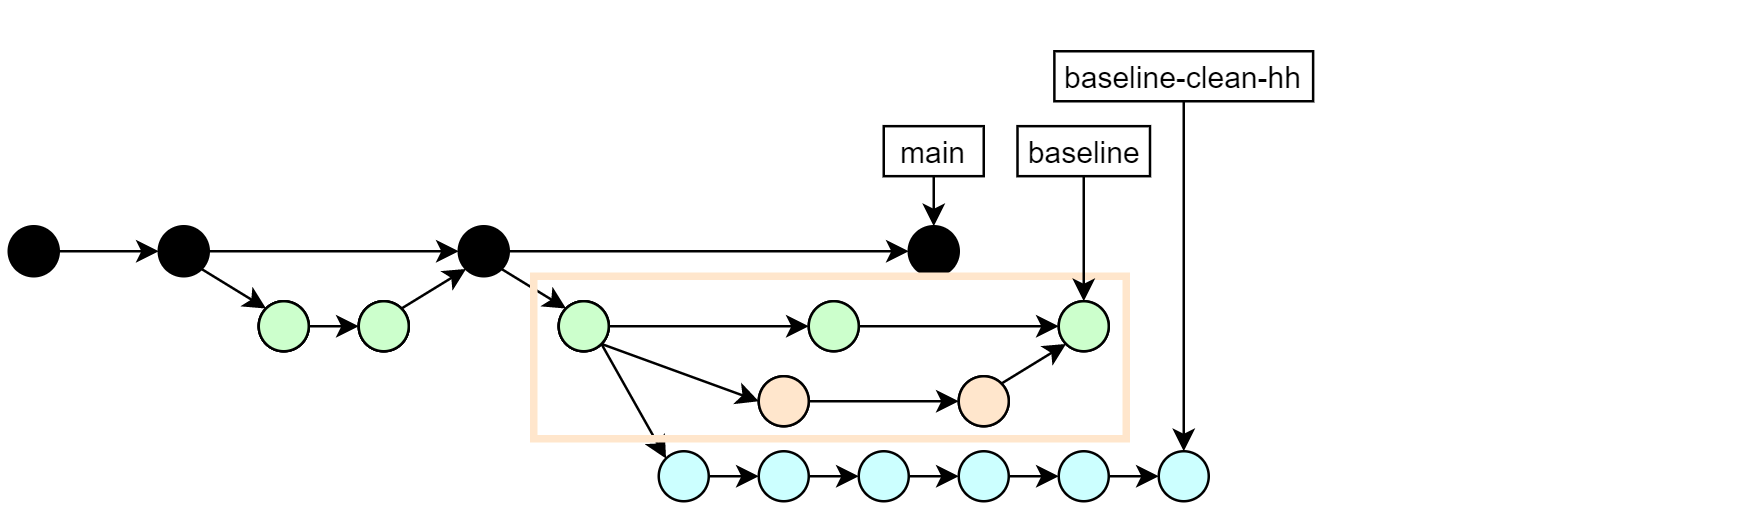
\includegraphics[width=\textwidth]{./img/dime-gitflow-network-2-4.png}
		\end{figure}
	\end{minipage}

	\vspace{-.5cm}
	\begin{minipage}[t][5cm][t]{\textwidth}
		\begin{itemize}
			\setlength\itemsep{.5em}
			\item The branch \texttt{baseline-clean-exp} was
			approved in the last step in the work stage and
			was merged and deleted in the merge stage.
			\item The orange box is one \textit{branch-PR-merge} cycle.
		\end{itemize}
	\end{minipage}
\end{frame}

\begin{frame}
	\frametitle{Merge a feature branch}

	\vspace{-.5cm}
	\begin{minipage}[t][5cm][t]{\textwidth}
		\begin{figure}
			\centering
			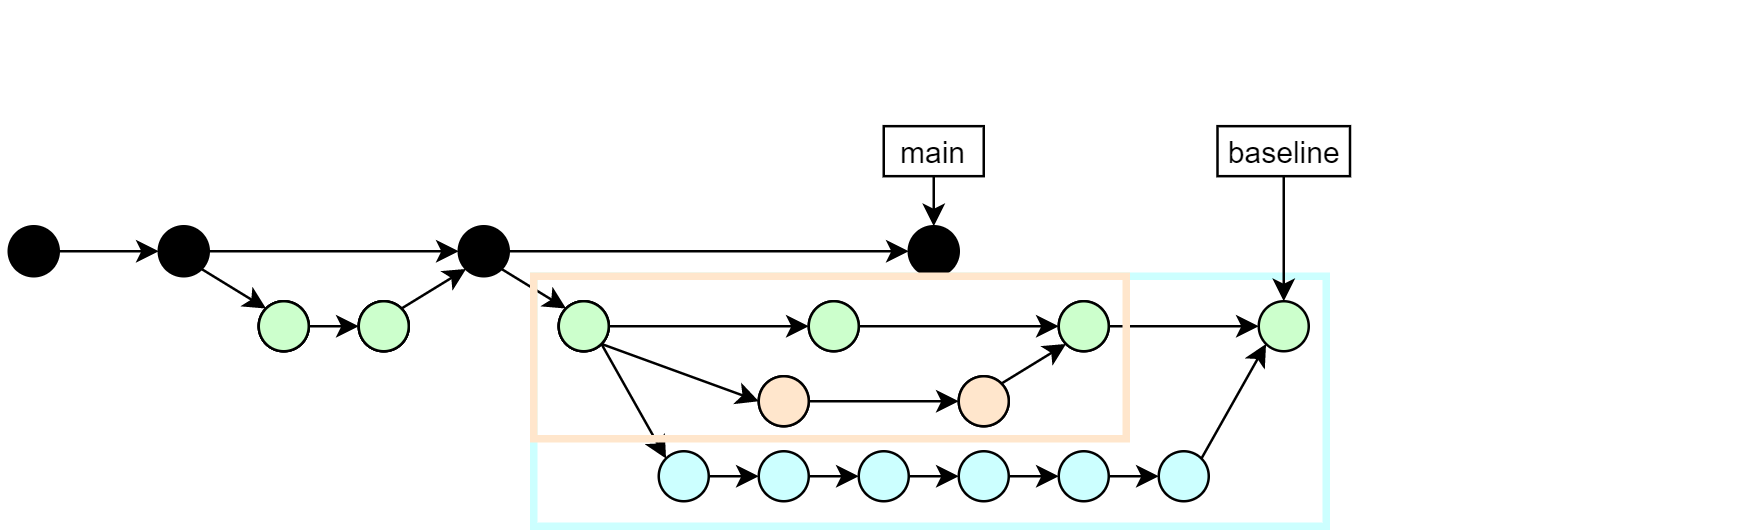
\includegraphics[width=\textwidth]{./img/dime-gitflow-network-2-5.png}
		\end{figure}
	\end{minipage}

	\vspace{-.5cm}
	\begin{minipage}[t][5cm][t]{\textwidth}
		\begin{itemize}
			\setlength\itemsep{.5em}
			\item The branch \texttt{baseline-clean-hh} was then
			also approved in the last step in the work stage and
			was merged and deleted in the merge stage.
			\item The blue box is also a \textit{branch-PR-merge} cycle.
		\end{itemize}
	\end{minipage}
\end{frame}

\begin{frame}
	\frametitle{Merge a develop branch}

	\vspace{-.5cm}
	\begin{minipage}[t][5cm][t]{\textwidth}
		\begin{figure}
			\centering
			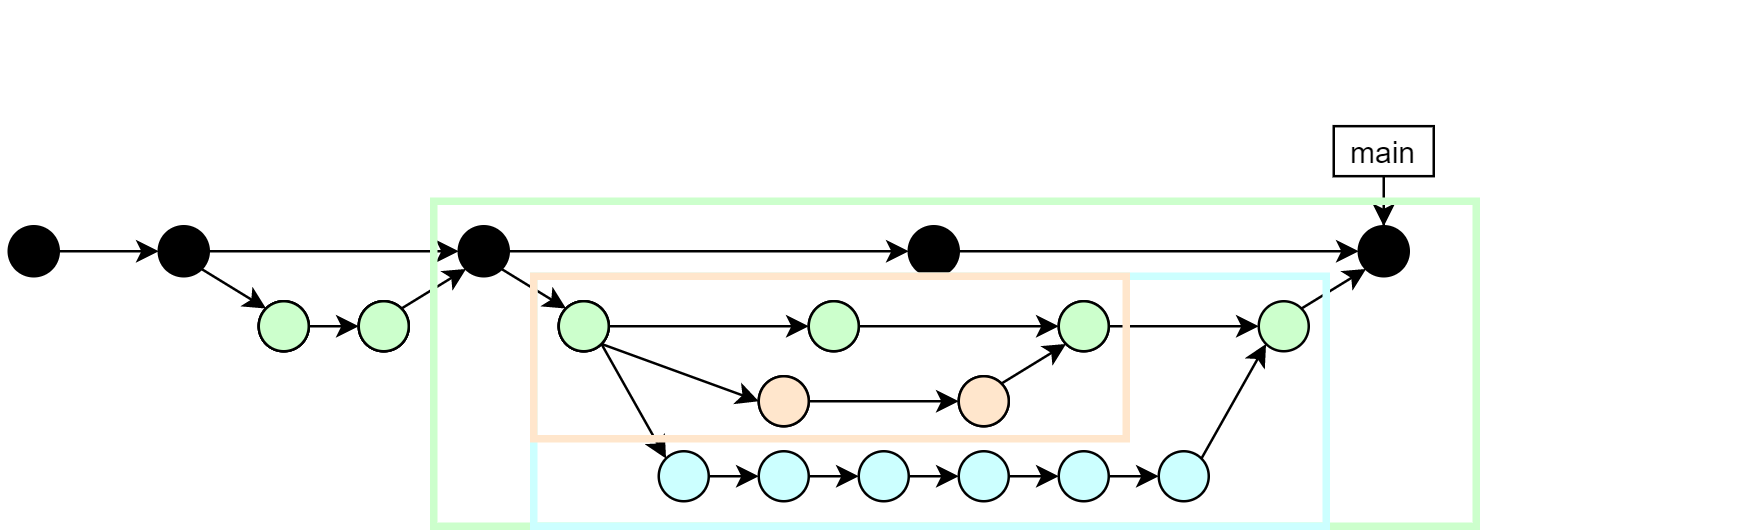
\includegraphics[width=\textwidth]{./img/dime-gitflow-network-2-6.png}
		\end{figure}
	\end{minipage}

	\vspace{-.5cm}
	\begin{minipage}[t][5cm][t]{\textwidth}
		\begin{itemize}
			\setlength\itemsep{.5em}
			\item Then the branch \texttt{baseline} is ready for a review
			- assign a reviewer - comment/suggest - accept/reject/discuss.
			\item The green box is also a \textit{branch-PR-merge} cycle.
			\item This network graph shows
			a nested \textit{branch-PR-merge} cycle.
		\end{itemize}
	\end{minipage}
\end{frame}

\begin{frame}
	\frametitle{Nest cycles in the work stage}
	\begin{columns}[c]
		
		\column{.4\textwidth} % Left column and width
		\begin{itemize}
			\setlength\itemsep{1em}
			\item \textit{Branch-PR-merge} cycles should be nested
			in the work stage.
			\item The \textit{develop} branch is kept
			in the \textit{Commit edits} step while
			the \textit{branch-PR-merge} cycles are completed
			for the feature branches.
			\item If needed, convert a \textit{feature} branch
			to a \textit{develop} branch here.
		\end{itemize}
		
		\column{.6\textwidth} % Right column and width
		\vspace{-.75cm}
		\begin{figure}
			\centering
			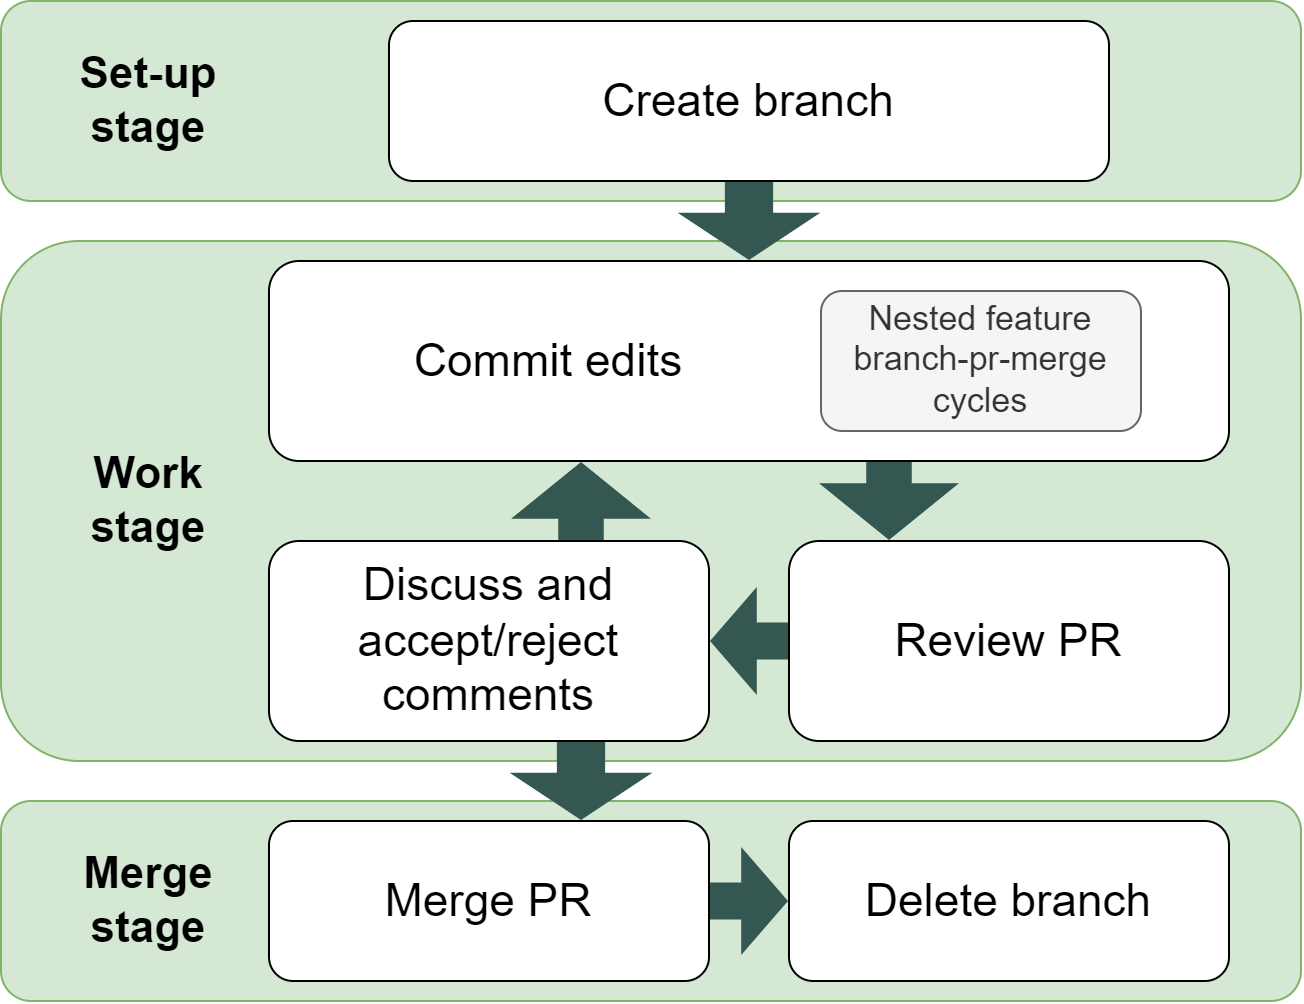
\includegraphics[width=\textwidth]{./img/nested-branch-pr-merge-cycle.png}
		\end{figure}
	\end{columns}
\end{frame}

\begin{frame}
	\frametitle{Work directly in main/develop}

	\vspace{-.5cm}
	\begin{minipage}[t][5cm][t]{\textwidth}
		\begin{figure}
			\centering
			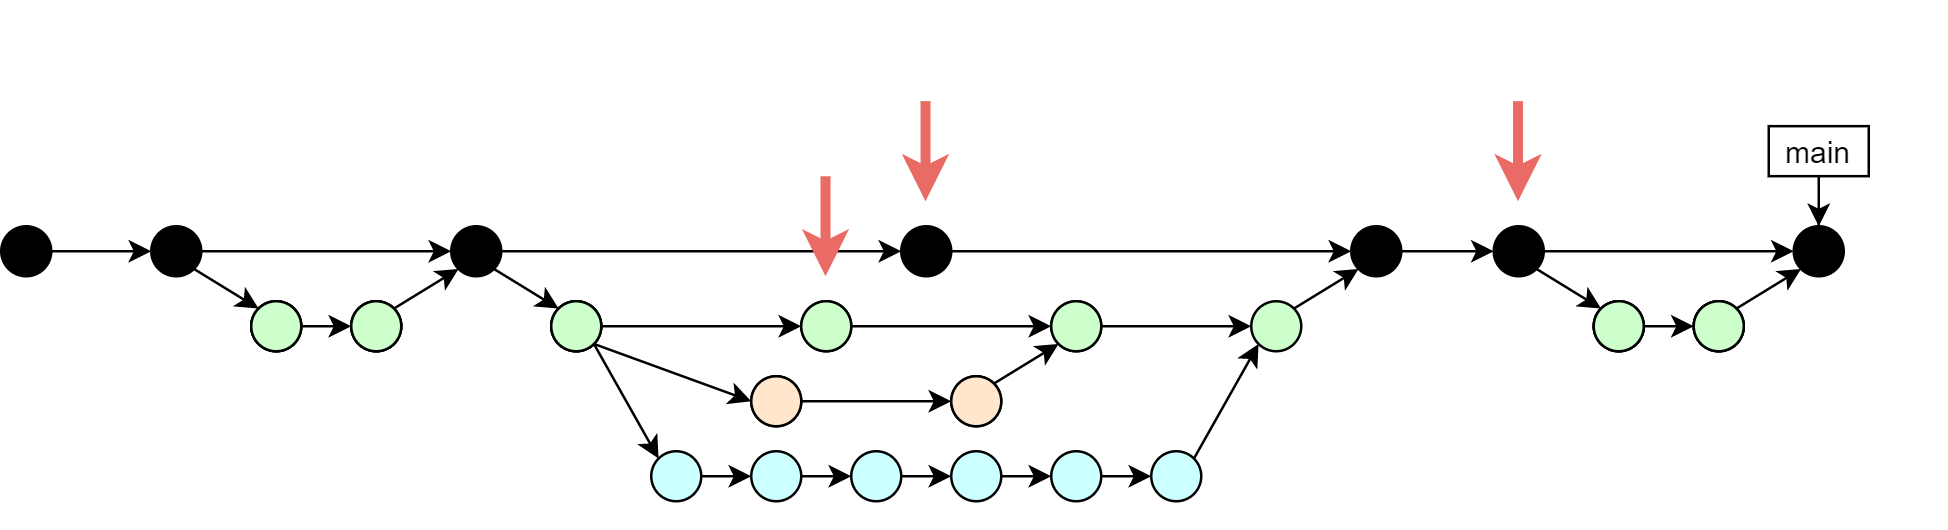
\includegraphics[width=\textwidth]{./img/dime-gitflow-network-workdirectly.png}
		\end{figure}
	\end{minipage}

	\vspace{-.5cm}
	\begin{minipage}[t][5cm][t]{\textwidth}
		\begin{itemize}
			\setlength\itemsep{.5em}
			\item <1->When would it be ok to work
			directly on a \textit{main}/\textit{develop} branch?
			- see red arrows
			\item <2->When updating documentation!
			\begin{itemize}
				\setlength\itemsep{.5em}
				\item <2->Documentation about the repo
				in the \textit{main} branch.
				\item <2->Documentation about the high-level task
				in the \textit{develop} branch.
			\end{itemize}
		\end{itemize}
	\end{minipage}
\end{frame}

\begin{frame}
	\frametitle{The network graph}

	\vspace{-.5cm}
	\begin{minipage}[t][5cm][t]{\textwidth}
		\begin{figure}
			\centering
			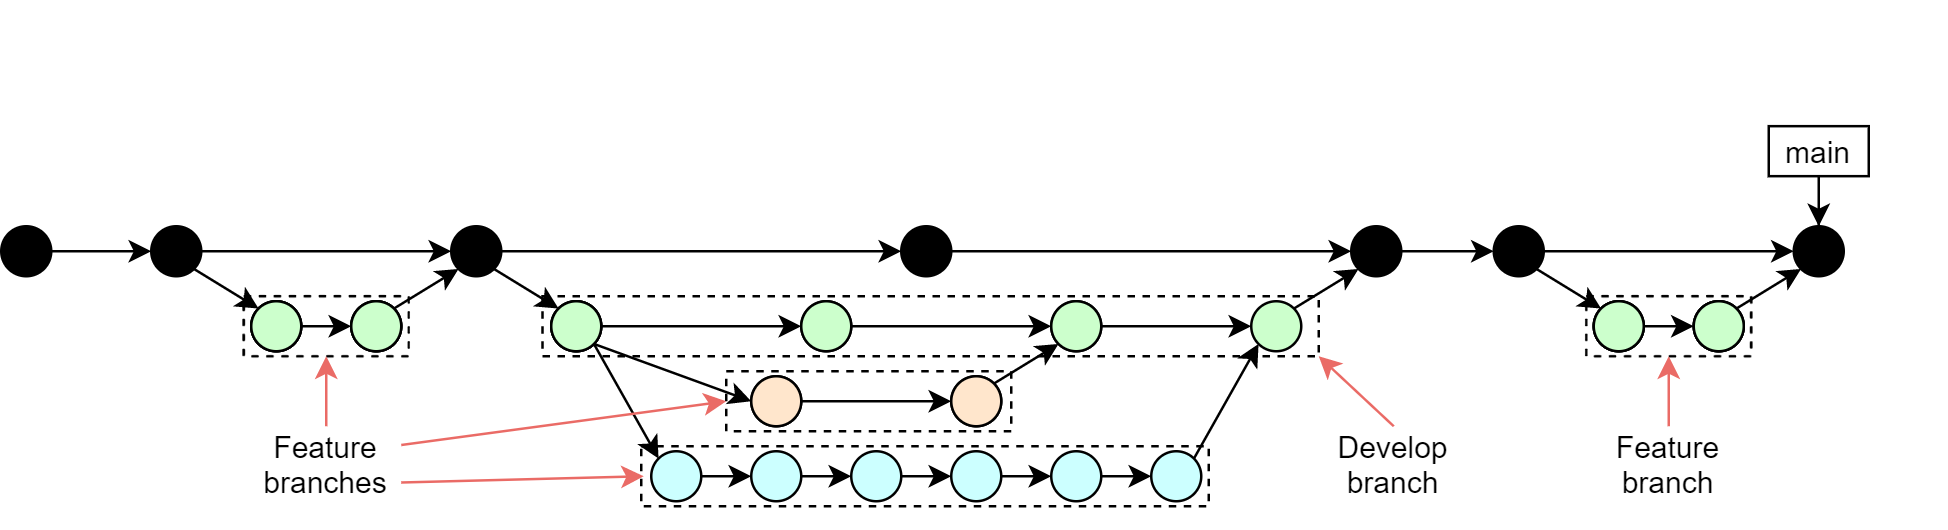
\includegraphics[width=\textwidth]{./img/dime-gitflow-network-names.png}
		\end{figure}
	\end{minipage}

	\vspace{-1cm}
	\begin{minipage}[t][5cm][t]{\textwidth}
		\begin{itemize}
			\setlength\itemsep{.4em}
			\item There is no difference to git between
			different Gitflow types of branches
			- the only difference is how team members use them.
			\begin{itemize}
				\setlength\itemsep{.5em}
				\item \textbf{Main branch}:
				The branch where all branches originate from.
				\item \textbf{Develop branch}:
				Non-\textit{main} branch with \textit{feature} branches.
				\item \textbf{Feature branch}:
				Branches of the \textit{main} branch or
				\textit{develop} branches with no other branches from it.
			\end{itemize}
		\end{itemize}
	\end{minipage}
\end{frame}

\begin{frame}
	\frametitle{ Exercise: Apply the Gitflow philosofy}
	\begin{itemize}
		\item \textbf{Objective:} Apply Gitflow concepts by managing genre-specific development branches and personal feature branches.
		\item \textbf{Branch Structure:}
		    \begin{itemize}
		        \item \textbf{Develop Branches:} Pre-created, genre-specific branches (e.g., \textit{rock}, \textit{pop}, \textit{metal}). These mimic the "develop" branches in the Gitflow model.
		        \item \textbf{Feature Branches:} Each participant creates a new branch from their chosen genre's develop branch, naming it \textit{genre\_your\_name} (e.g., \textit{rock\_alice}). This is where individual work occurs.
		        \item \textbf{Main Branch:} The central branch from which all genre branches originate. This branch typically contains the consolidated and final version of the project.
            \end{itemize}
            \end{itemize}

          \end{frame}

          \begin{frame}
          \frametitle{ Exercise: Apply the Gitflow philosofy}
          \begin{itemize}
		 
		\item \textbf{Tasks:}
		\begin{enumerate}
			\item Choose a genre and create your feature branch from the respective genre's develop branch. Name your branch genre\_your\_name.
			\item Add a new song to the genre folder in your branch, commit the changes, and push them to GitHub.
			\item Open a pull request to merge your feature branch back into the develop branch for your chosen genre.
			\item Let's now explore \hyperlink{https://github.com/dime-wb-trainings/lyrics-msfr24/network}{the network graph}.
		\end{enumerate}
		\item \textbf{Discussion:}
		    \begin{itemize}
		        \item Reflect on how this branching strategy can be analogous to task management in complex projects, such as field research or software development.
		        \item Discuss the benefits of organizing work into specific branches to maintain clarity and improve collaboration.
		    \end{itemize}
	    \end{itemize}
      

\end{frame}


\begin{frame}
	\frametitle{Thank you!}
	\huge\centering \textbf{Questions?}

\end{frame}

\begin{frame}{Useful links}
	\begin{itemize}
	  \item All DIME Analytics GitHub trainings: \trainingURL{https://osf.io/e54gy/}
	  \item Other DIME Analytics GitHub resources: \trainingURL{https://github.com/worldbank/dime-github-trainings}. For example:
		\begin{itemize}
			\item DIME Analytics GitHub Templates (for example .gitignore): \trainingURL{https://github.com/worldbank/dime-github-trainings/tree/master/GitHub-resources/DIME-GitHub-Templates}
			\item DIME Analytics GitHub Roles: \trainingURL{https://github.com/worldbank/dime-github-trainings/blob/master/GitHub-resources/DIME-GitHub-Roles/DIME-GitHub-roles.md}
		\end{itemize}
		\item Markdown cheat sheet (how to format text on GitHub.com):  \trainingURL{https://www.markdownguide.org/cheat-sheet/}
		\item DIME GitHub Account admin info and instructions: \trainingURL{https://github.com/dime-worldbank/dime-account-admin}
	\end{itemize}
\end{frame}

\end{document} 